\documentclass[12pt]{article} 
\usepackage[utf8]{inputenc}
\usepackage[margin=2.5cm]{geometry} % decrease the margin size

\usepackage{hyperref} % to include weblinks

\usepackage{graphicx} % handle images and figures
\usepackage{placeins} % to control placement of figures
\usepackage{subcaption}

\usepackage{amsmath} % general package for writing math
\usepackage{amsfonts} % math fonts for obscure symbols

\usepackage[version=4]{mhchem} % chemistry notation

\usepackage[nottoc]{tocbibind}
\usepackage[backend=biber,dateabbrev=false]{biblatex} % package for handling references
\addbibresource{references.bib}
\usepackage{csquotes}

\usepackage{fancyhdr}

\setlength{\parindent}{0pt} % remove indentation at the beginning of pargraphs

\begin{document}

\pagestyle{fancy}
\setlength{\headheight}{15pt}
\fancyhead[L]{X-Ray Diffraction}
\fancyhead[R]{Louis-Hendrik Barboutie, Rajon Bhuyan}

\begin{titlepage}
    \begin{center}
        \vspace*{1cm}
        \Huge
        \textbf{X-Ray Diffraction}
        
        \vspace{0.5cm}
        \LARGE
        Physikalisches Praktikum für Fortgeschrittene I
        
        \vspace{1.5cm}
        \textbf{Louis-Hendrik Barboutie and Rajon Bhuyan} \newline
        \textbf{7016306 \& 7029677}
        
        \vspace{0.5cm}
        \Large 
        Supervisor: Dipl.-Ing. Jörg Schmauch
        
        \vfill

        
\includegraphics[width=0.4\textwidth]{logo_uni.png}
        
        \Large
        08$^{\underline{\text{th}}}$ December 2022
    \end{center}
\end{titlepage}

\tableofcontents
\newpage

\section{Theory}

\subsection{Bragg's law}

Bragg's law is given as:
\begin{equation}
    2d \sin(\theta) = n \lambda
    \label{eq:Bragg1}
\end{equation}

Using the results from problem 1, it can be rewritten for cubic lattices as:
\begin{equation}
    \frac{2a}{\sqrt{h^2 + k^2 + l^2}} \sin( \theta ) = n \lambda
    \label{eq:Bragg2}
\end{equation}

\subsection{Lattice constant}

Rearranging eq. \ref{eq:Bragg2} we get:
\begin{equation}
    a = \frac{n \lambda}{2 \sin(\theta)}\sqrt{h^2 + k^2 + l^2}
    \label{eq:LatticeConstant2}
\end{equation}

The calculated lattice constant is linked to the true lattice constant by the relation (see \cite{LabGuideXRD} for the derivation):
\begin{equation}
    a = a_0 - \left( a_0 \frac{\tilde{d}}{r} \right) \frac{\cos^2(\theta)}{\sin(\theta)}
    \label{eq:LatticeConstant1}
\end{equation}



\subsection{Peak broadening}

\subsubsection{Lorentzian profile}

The total peak broadening for a Lorentzian is given by the sum of the broadening due to the  different sources:
\begin{equation}
    \delta(2\theta)_{total} = \delta(2\theta)_{inst} + \delta(2\theta)_{size} + \delta(2\theta)_{strain} 
\end{equation}

Assuming that the instrumental broadening is independent of the strain and size broadening, we can then link the crystallite size $D$ and strain $e$ by the following equation:
\begin{equation}
    \delta s = \frac{6}{5D} + 2 e s
    \label{eq:LorentzianStrainSize}
\end{equation}
Where we performed the change in variables $s = \frac{2 \sin(\theta)}{\lambda}$ and $\delta s = \delta(2\theta)_{total} - \delta(2\theta)_{inst}$ is the corrected peak broadening corrected. The peak broadening is then given by:
\begin{equation}
    \delta s = \frac{\cos(\theta)}{\lambda}(\delta 2 \theta)_{corr}
\end{equation}



\subsubsection{Gaussian profile}

The total peak broadening for a Gaussian is given by the sum of the squares of the broadening due to the  different sources:
\begin{equation}
    [\delta(2\theta)_{total}]^2 = [\delta(2\theta)_{inst}]^2 + [\delta(2\theta)_{size}]^2 + [\delta(2\theta)_{strain}]^2 
\end{equation}

Assuming that the instrumental broadening is independent of the strain and size broadening, we can then link the crystallite size $D$ and strain $e$ by the following equation:
\begin{equation}
    (\delta s)^2 = \left( \frac{6}{5D} \right)^2 + (2e s)^2
    \label{eq:GaussianStrainSize}
\end{equation}

Where we performed the change in variables $s = \frac{2 \sin(\theta)}{\lambda}$ and $[\delta s]^2 = [\delta(2\theta)_{total}]^2 - [\delta(2\theta)_{inst}]^2$ is the corrected peak broadening corrected. The peak broadening is then given by:
\begin{equation}
    \delta s = \frac{\cos(\theta)}{\lambda}(\delta 2 \theta)_{corr}
\end{equation}



\newpage

\section{Results}

\subsection{Spectra}
Using the goniometer, we perform automated measurements of the intensity as a function of the scattering angle. The spectra we obtained are shown in fig. \ref{fig:ExperimentalSpectra}.

\begin{figure}[!ht]
    \begin{subfigure}{0.5\textwidth}
        \centering
        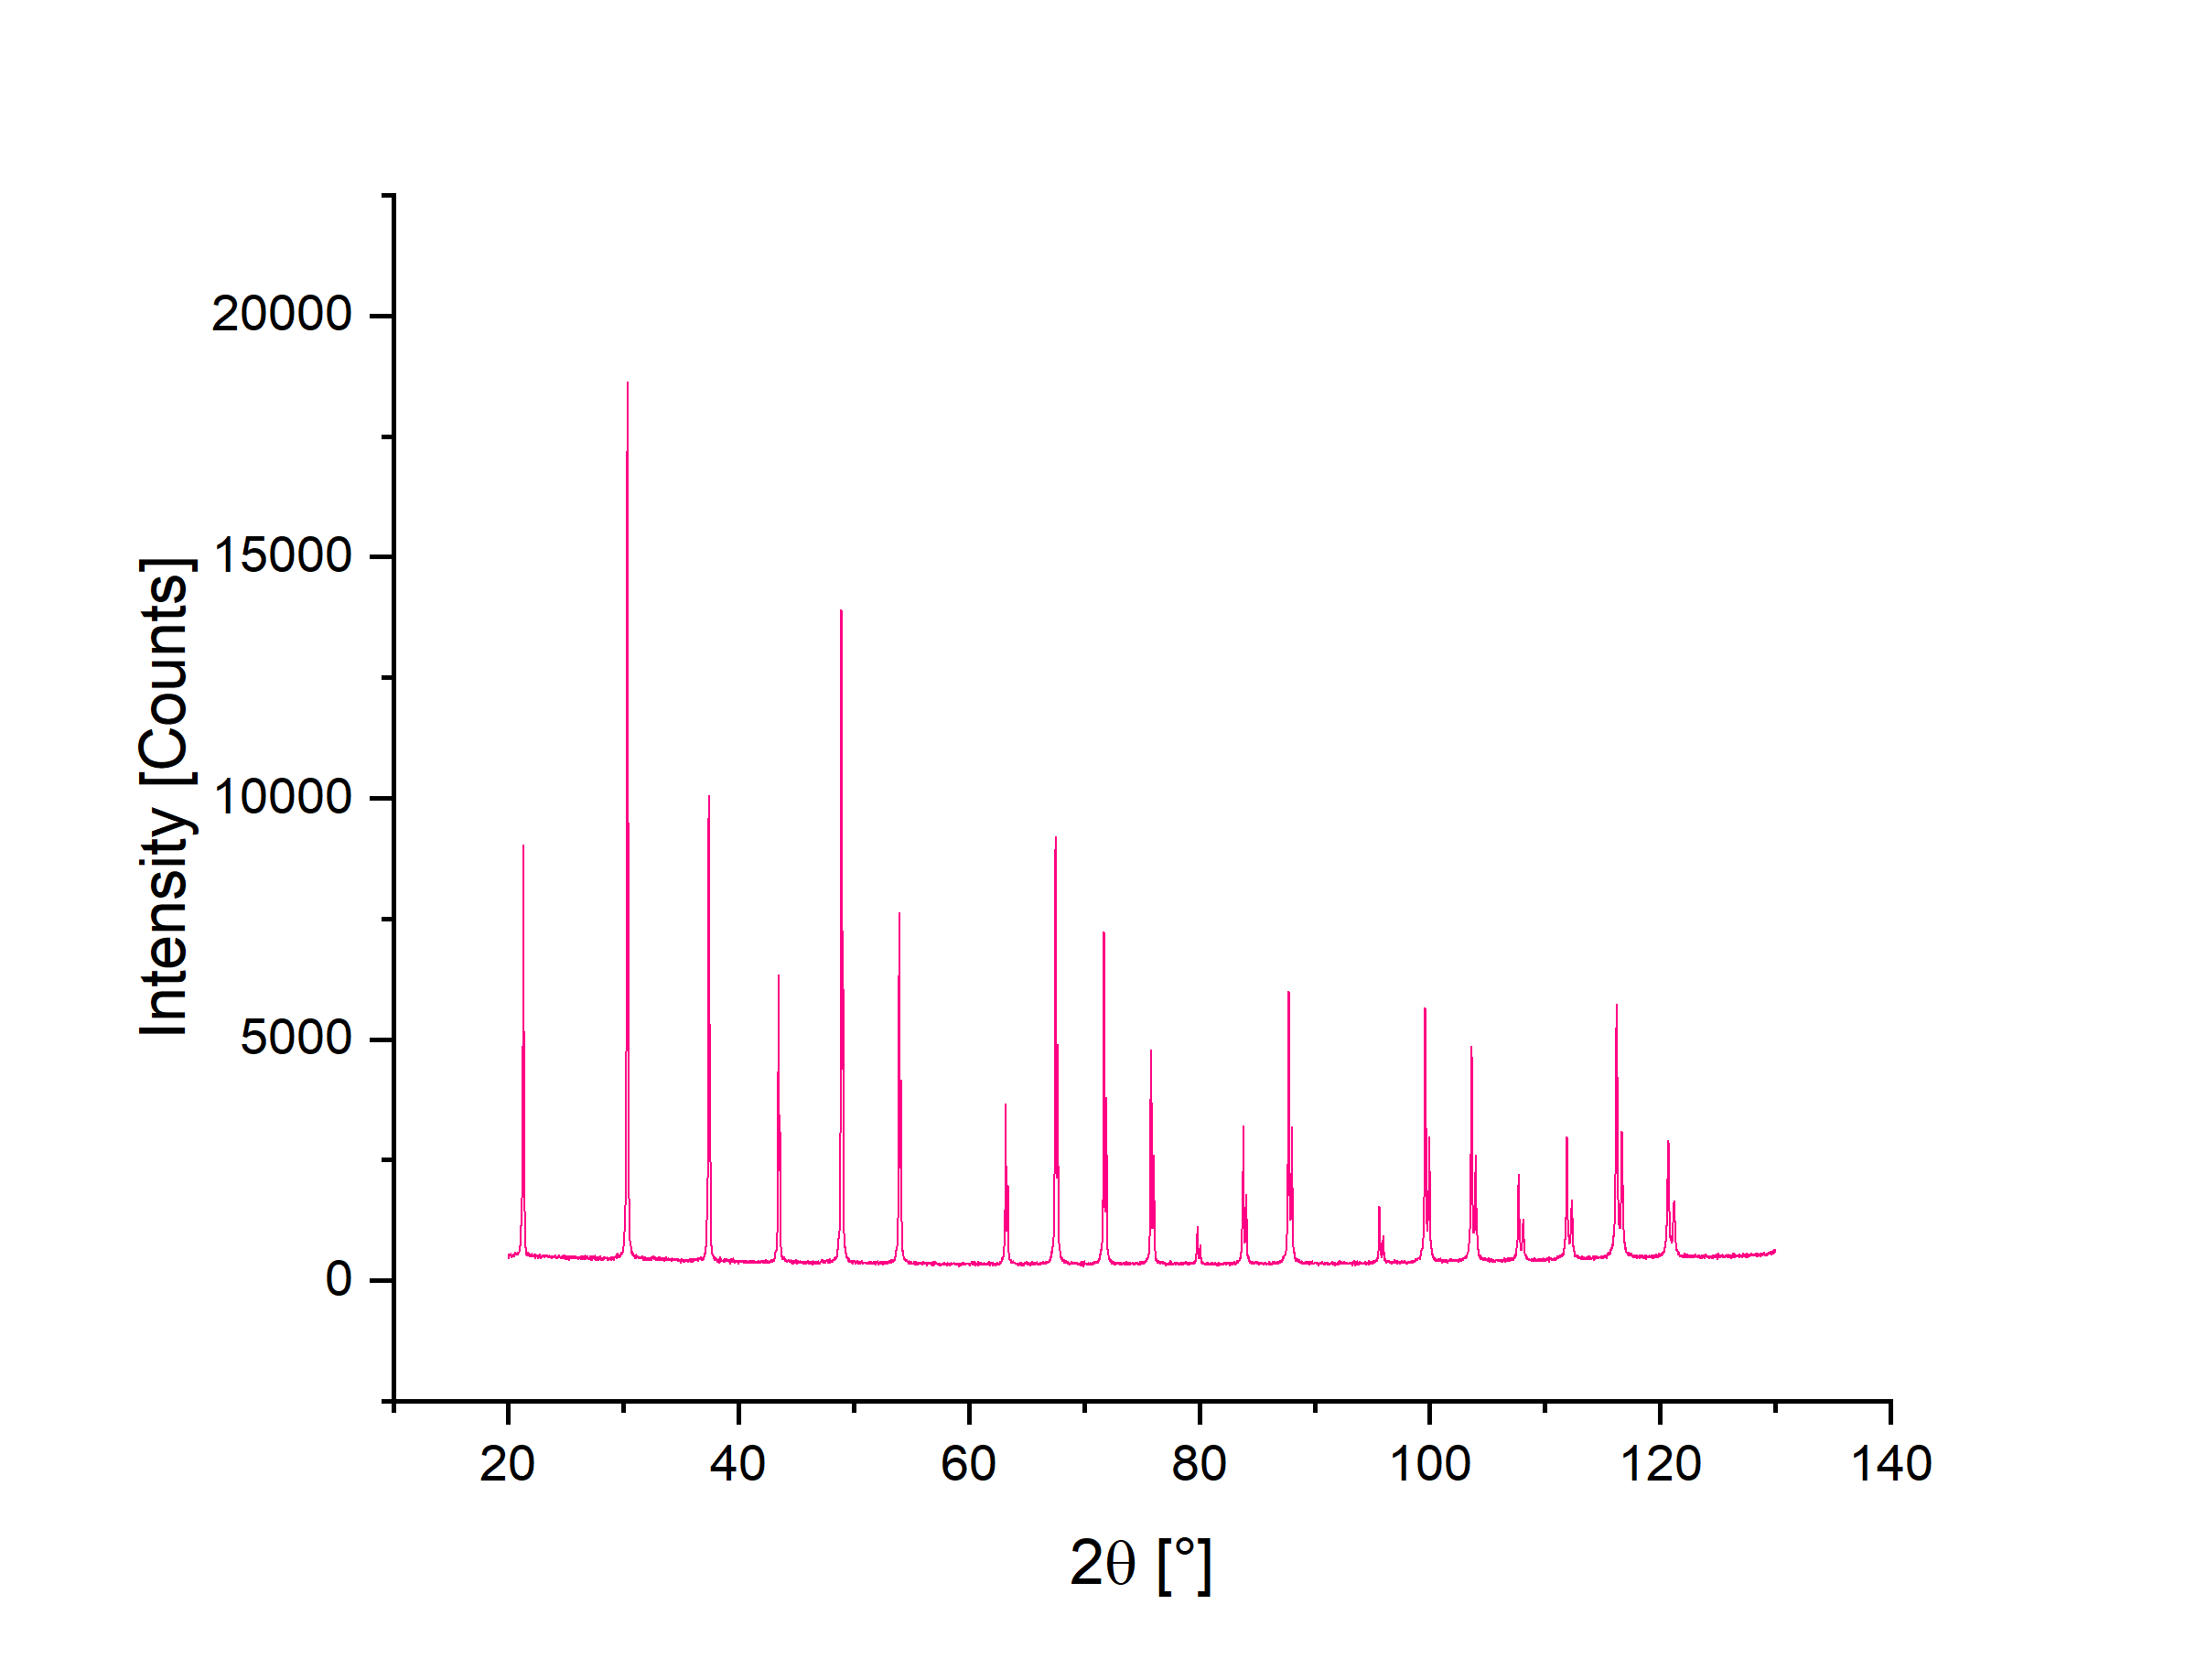
\includegraphics[width=\linewidth]{2_XRD/Graphics/Experiments/Spectra/Spectrum_LaB6.png}
        \caption{\ce{LaB6}}
    \end{subfigure}
    \begin{subfigure}{0.5\textwidth}
        \centering
        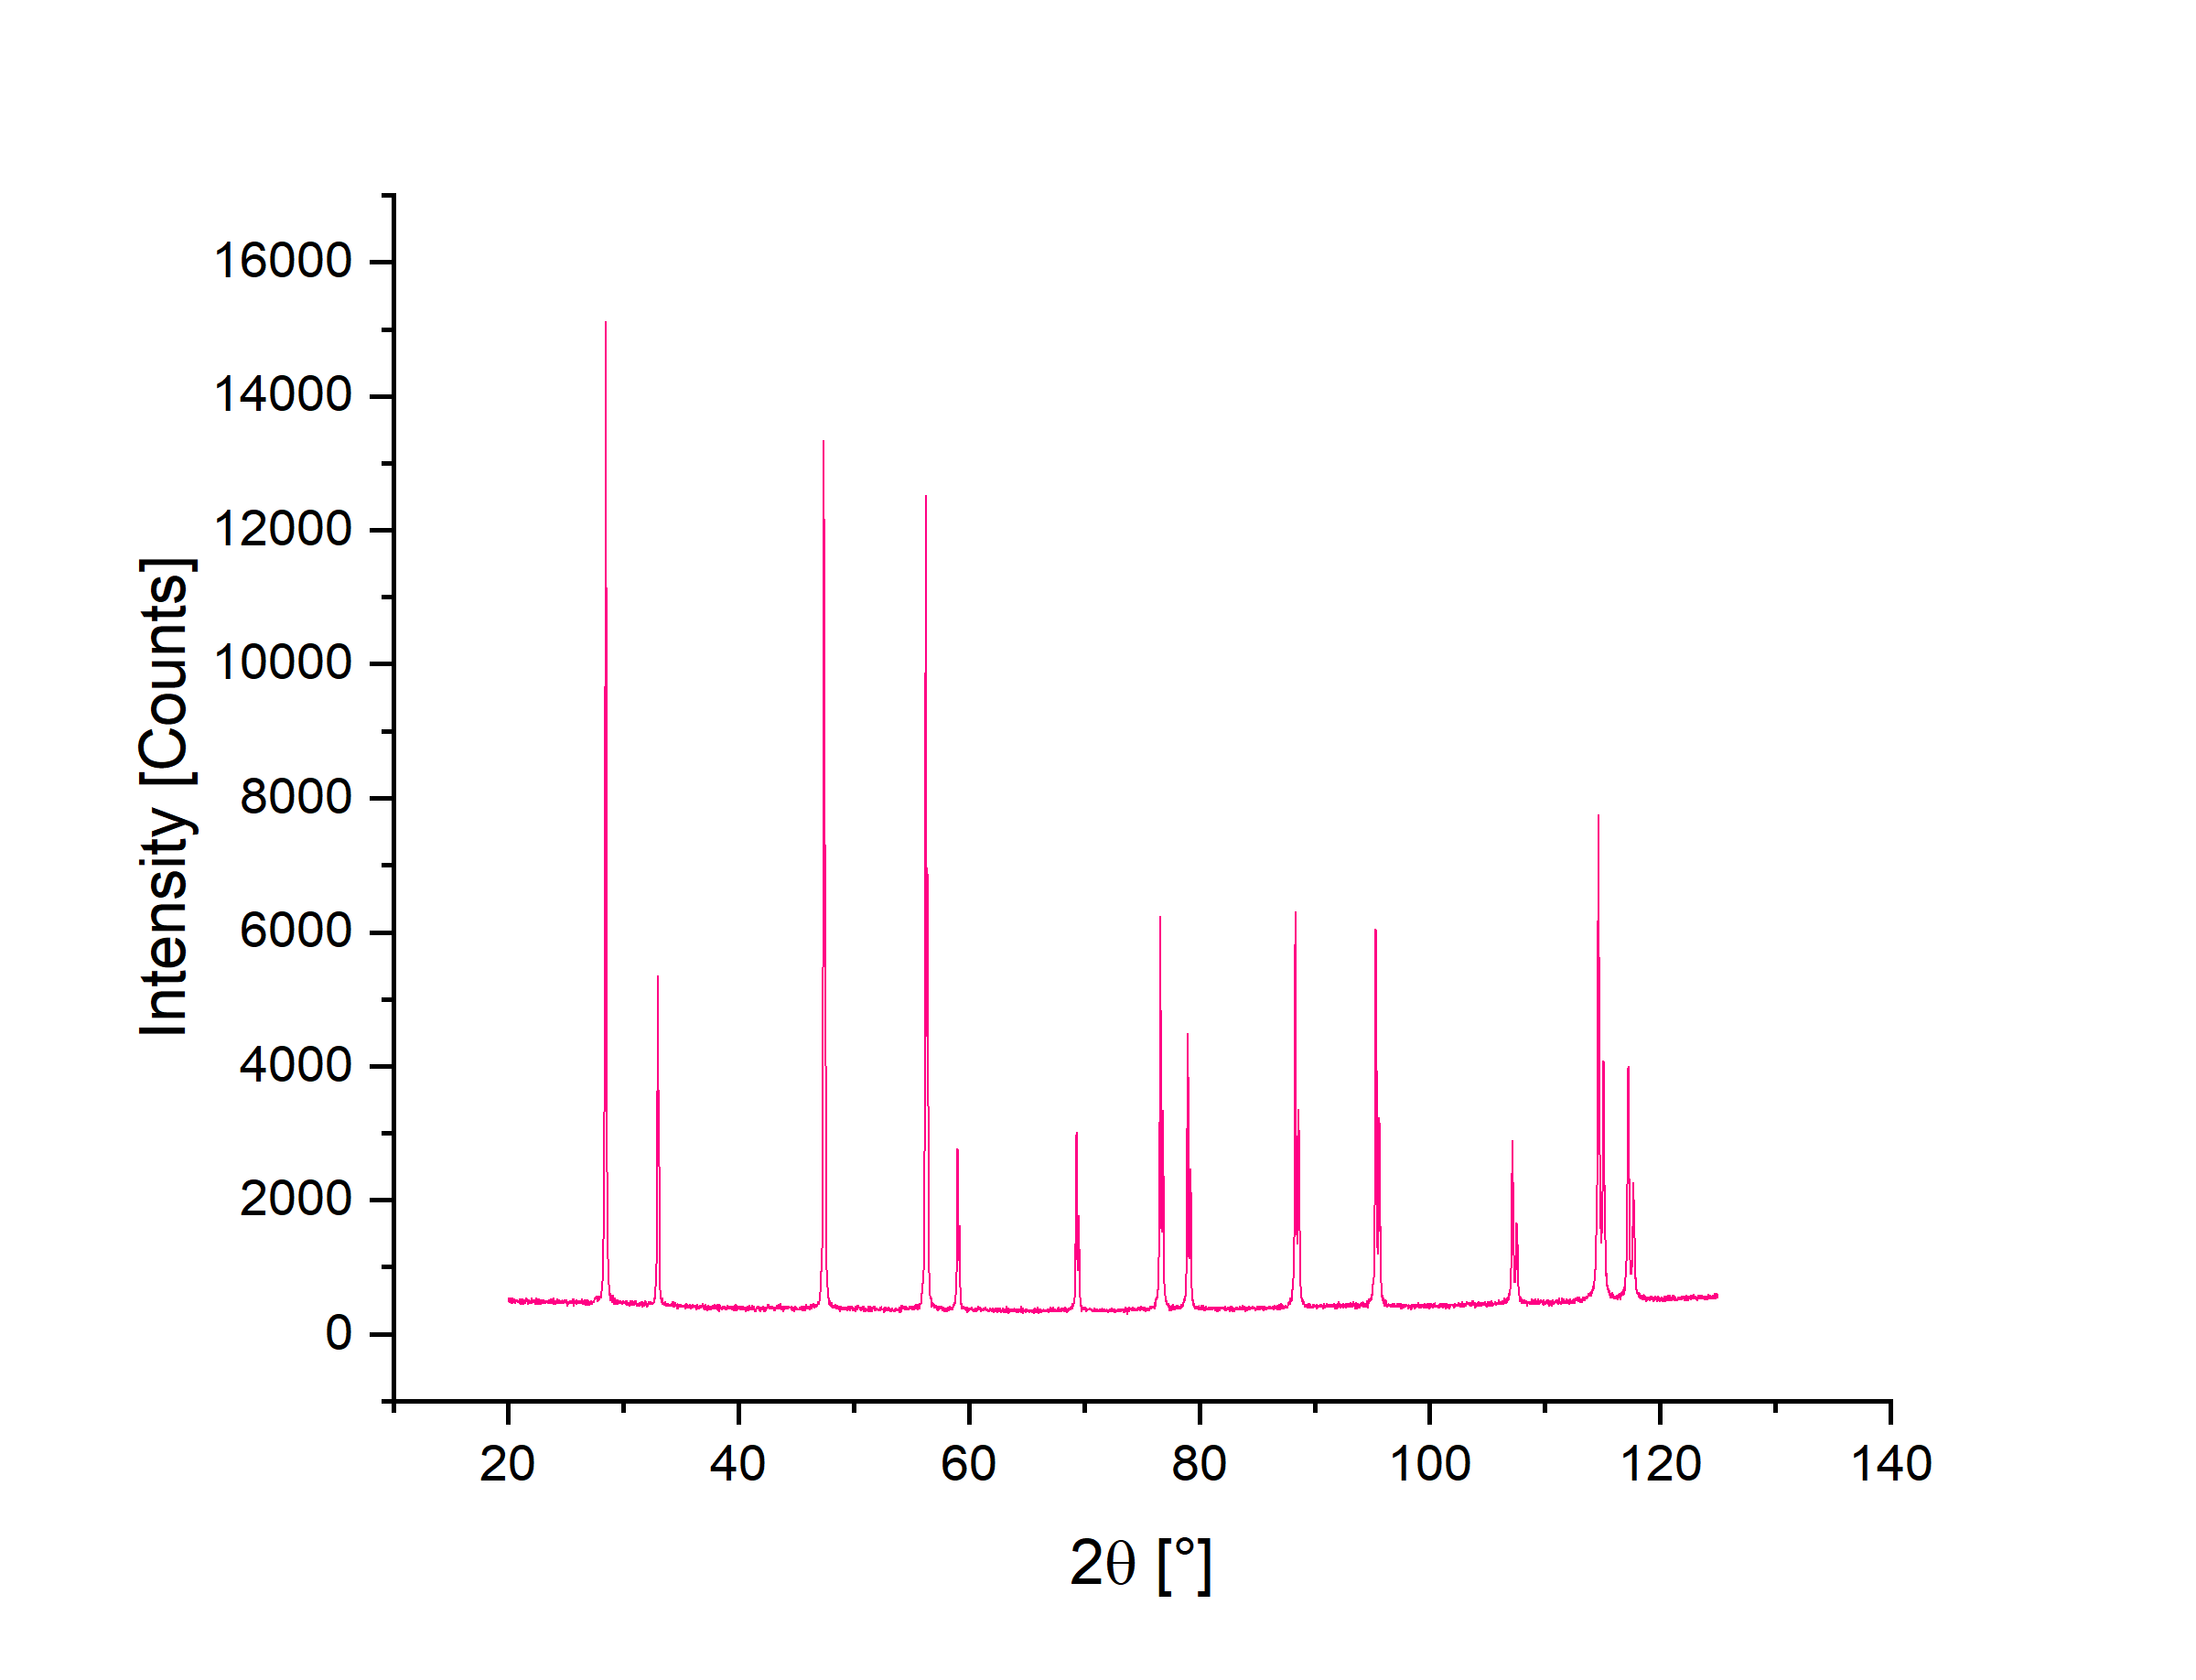
\includegraphics[width=\linewidth]{2_XRD/Graphics/Experiments/Spectra/Spectrum_CeO2_1.png}
        \caption{micro-crystalline \ce{CeO2}}
    \end{subfigure}

    \medskip
    
    \begin{subfigure}{0.5\textwidth}
        \centering
        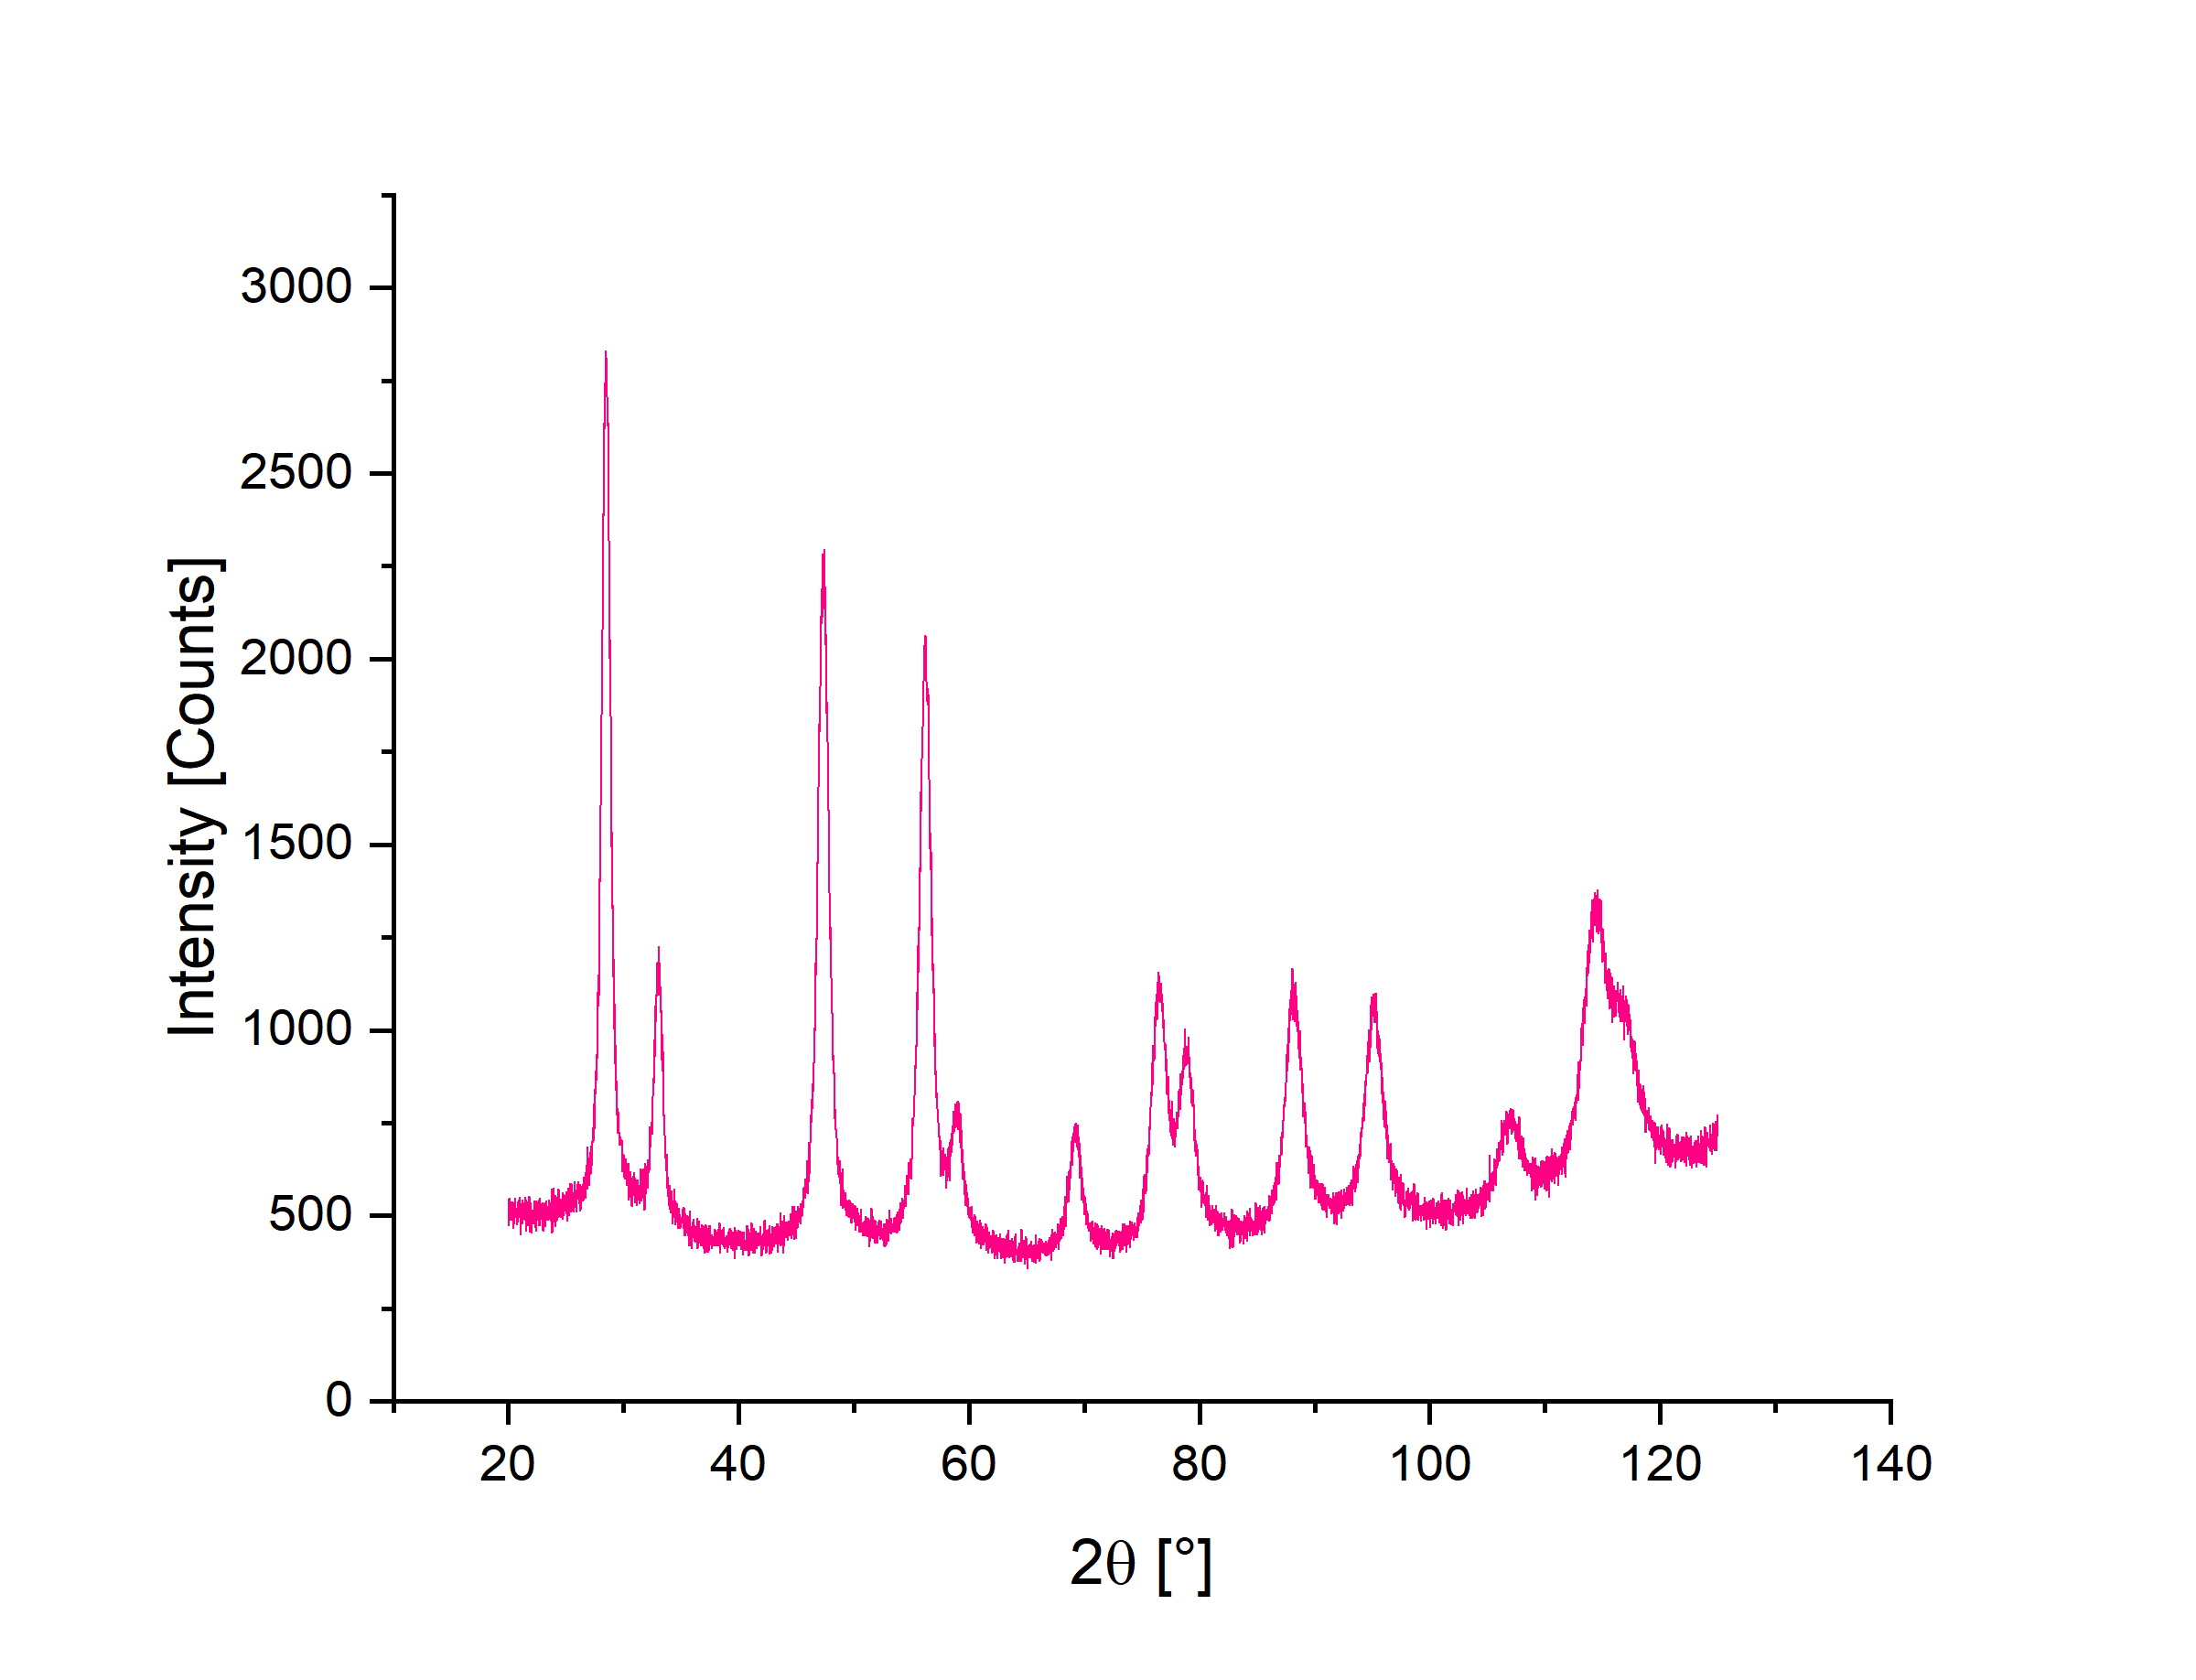
\includegraphics[width=\linewidth]{2_XRD/Graphics/Experiments/Spectra/Spectrum_CeO2_2.png}
        \caption{nano-crystalline \ce{CeO2}}
    \end{subfigure}
    \begin{subfigure}{0.5\textwidth}
        \centering
        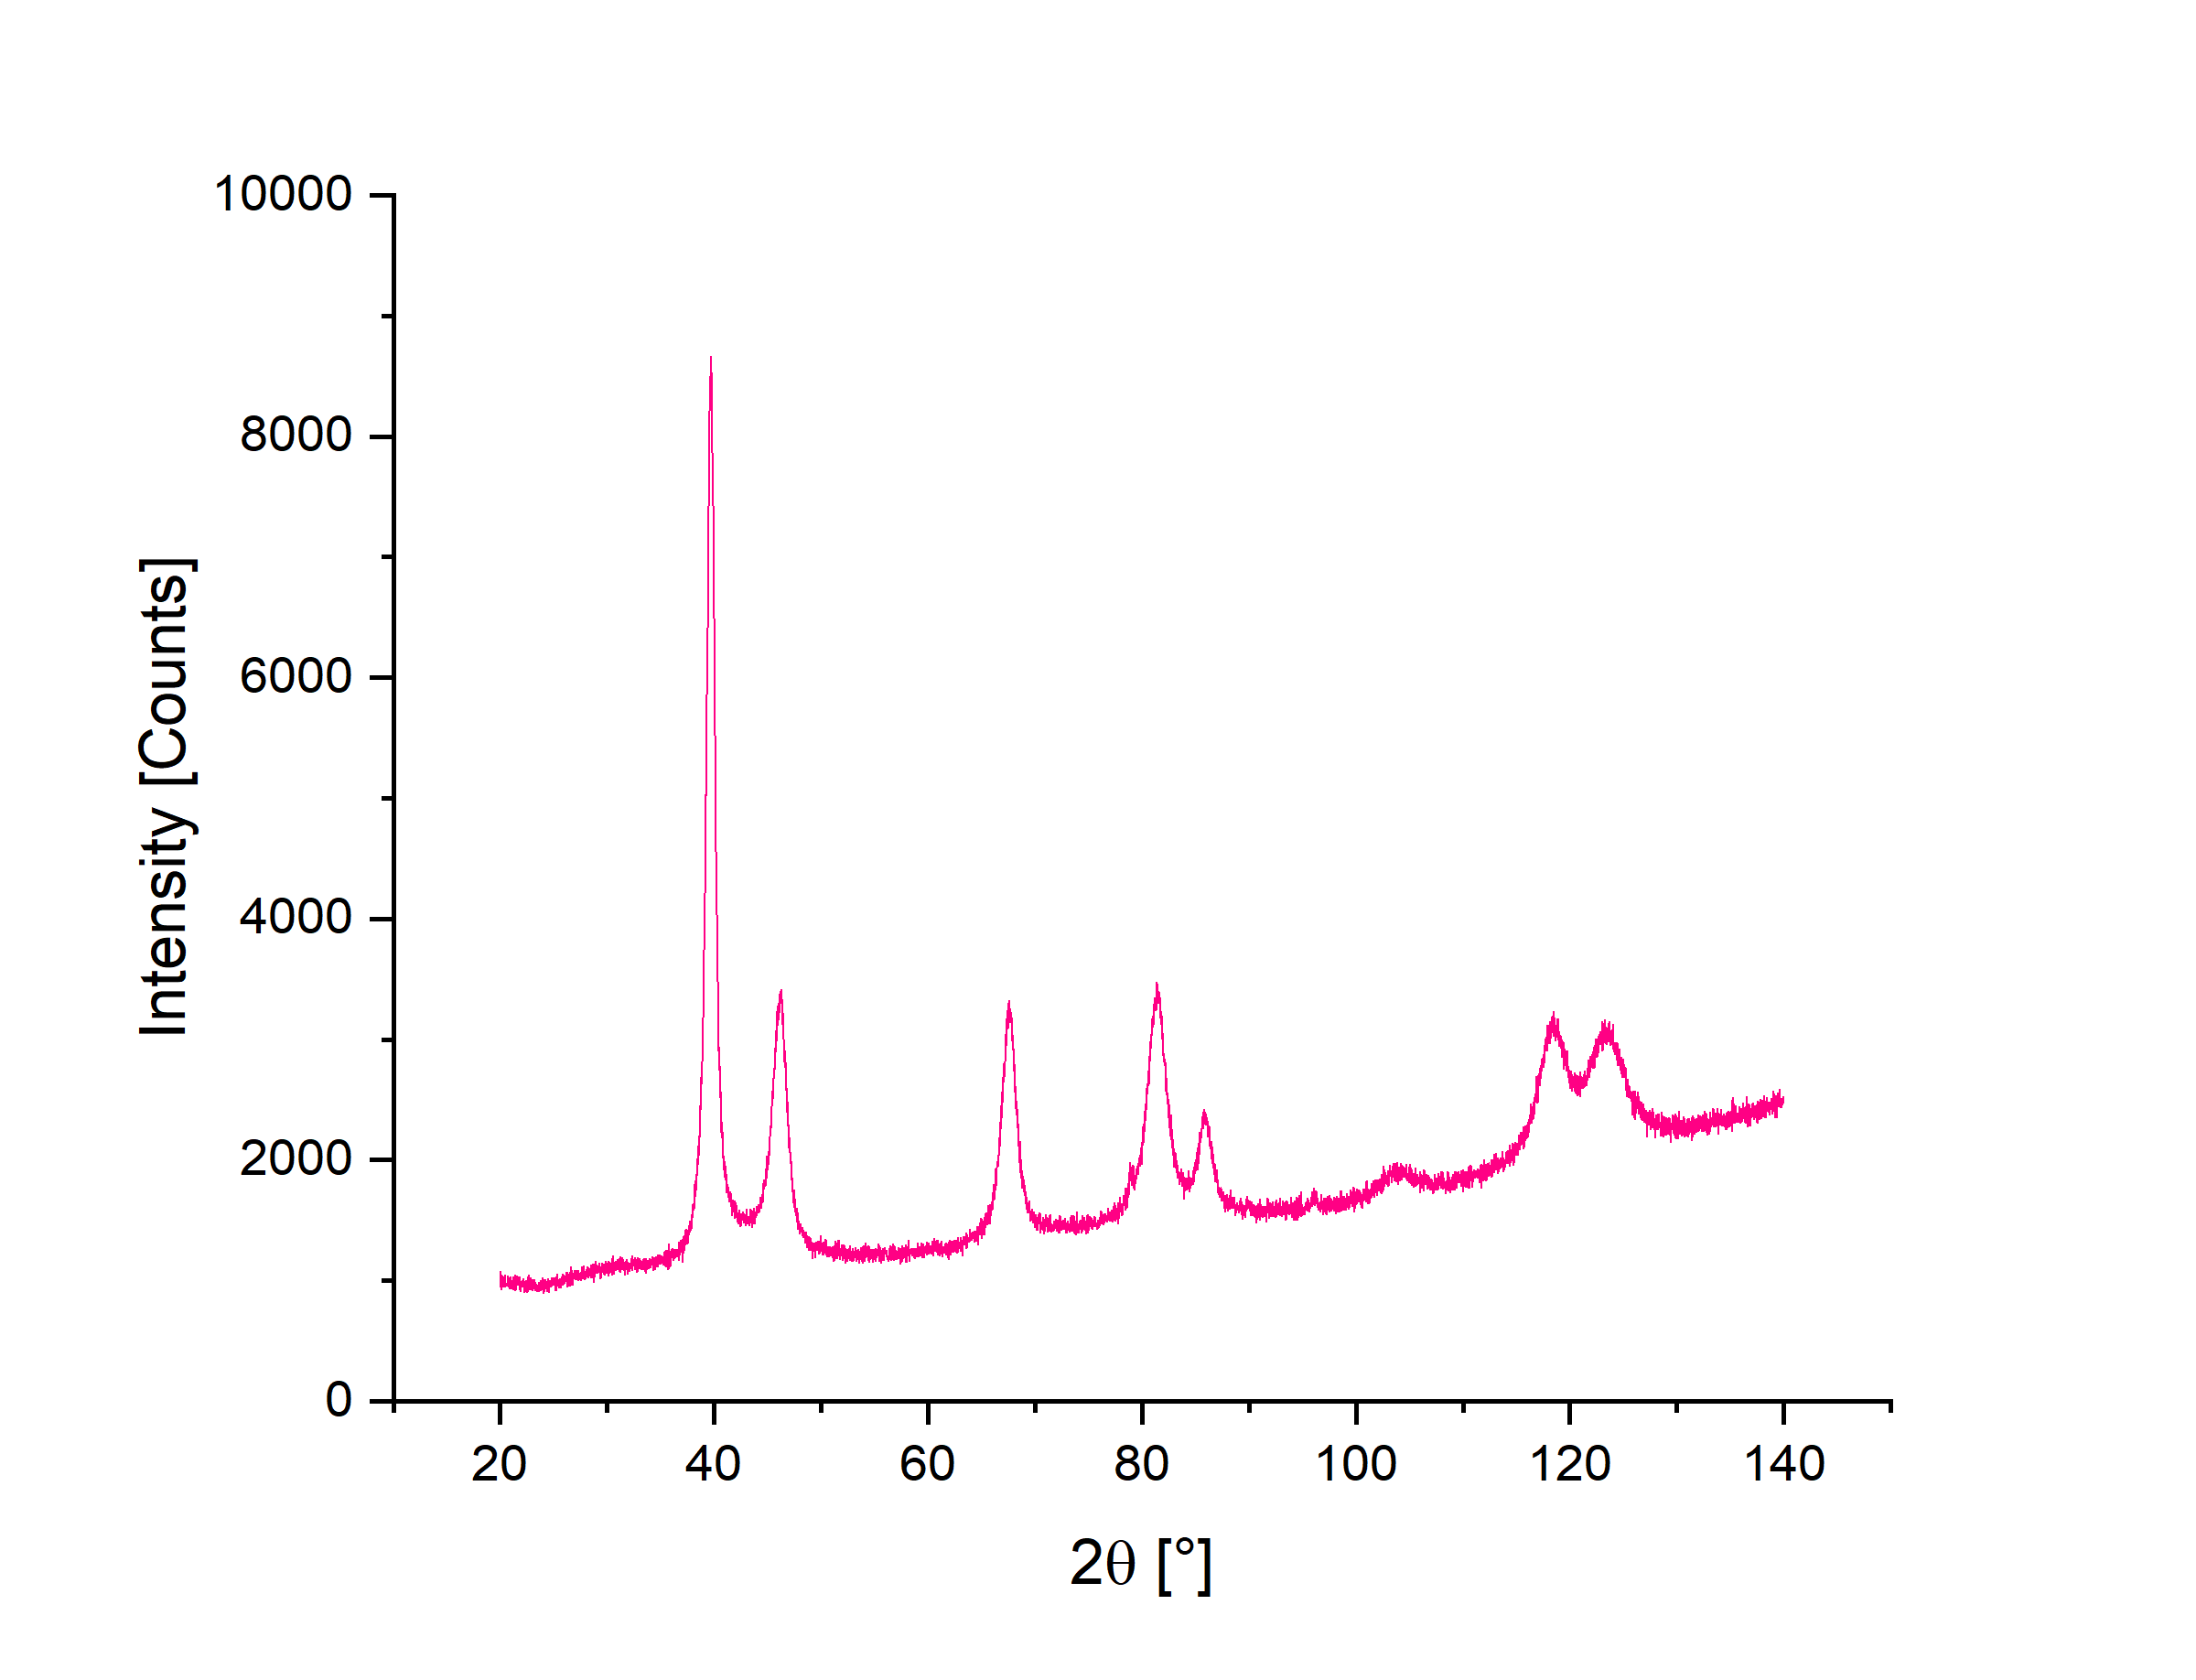
\includegraphics[width=\linewidth]{2_XRD/Graphics/Experiments/Spectra/Spectrum_Pd90Au10.png}
        \caption{\ce{Pd90Au10}}
    \end{subfigure}
    
    \caption{Experimental Spectra}
    \label{fig:ExperimentalSpectra}
\end{figure}

\subsection{Lattice constants}

Since we know the values of $(h,k,l)$ for each of the first eight peaks (see problem 2) and using eq. \ref{eq:LatticeConstant2}, we can calculate $a$. By eq. \ref{eq:LatticeConstant1} this yields a linear relationship and we can deduce the true value $a_0$ of the lattice constant as the intercept at origin. The plots of the resulting data for both \ce{CeO2} and the \ce{Pd90Au10} samples are presented in fig. \ref{fig:LatticeConstant_CeO2_1}, fig. \ref{fig:LatticeConstant_CeO2_2} and fig. \ref{fig:LatticeConstant_Pd90Au10}:

\begin{figure}[!ht]
    \centering
    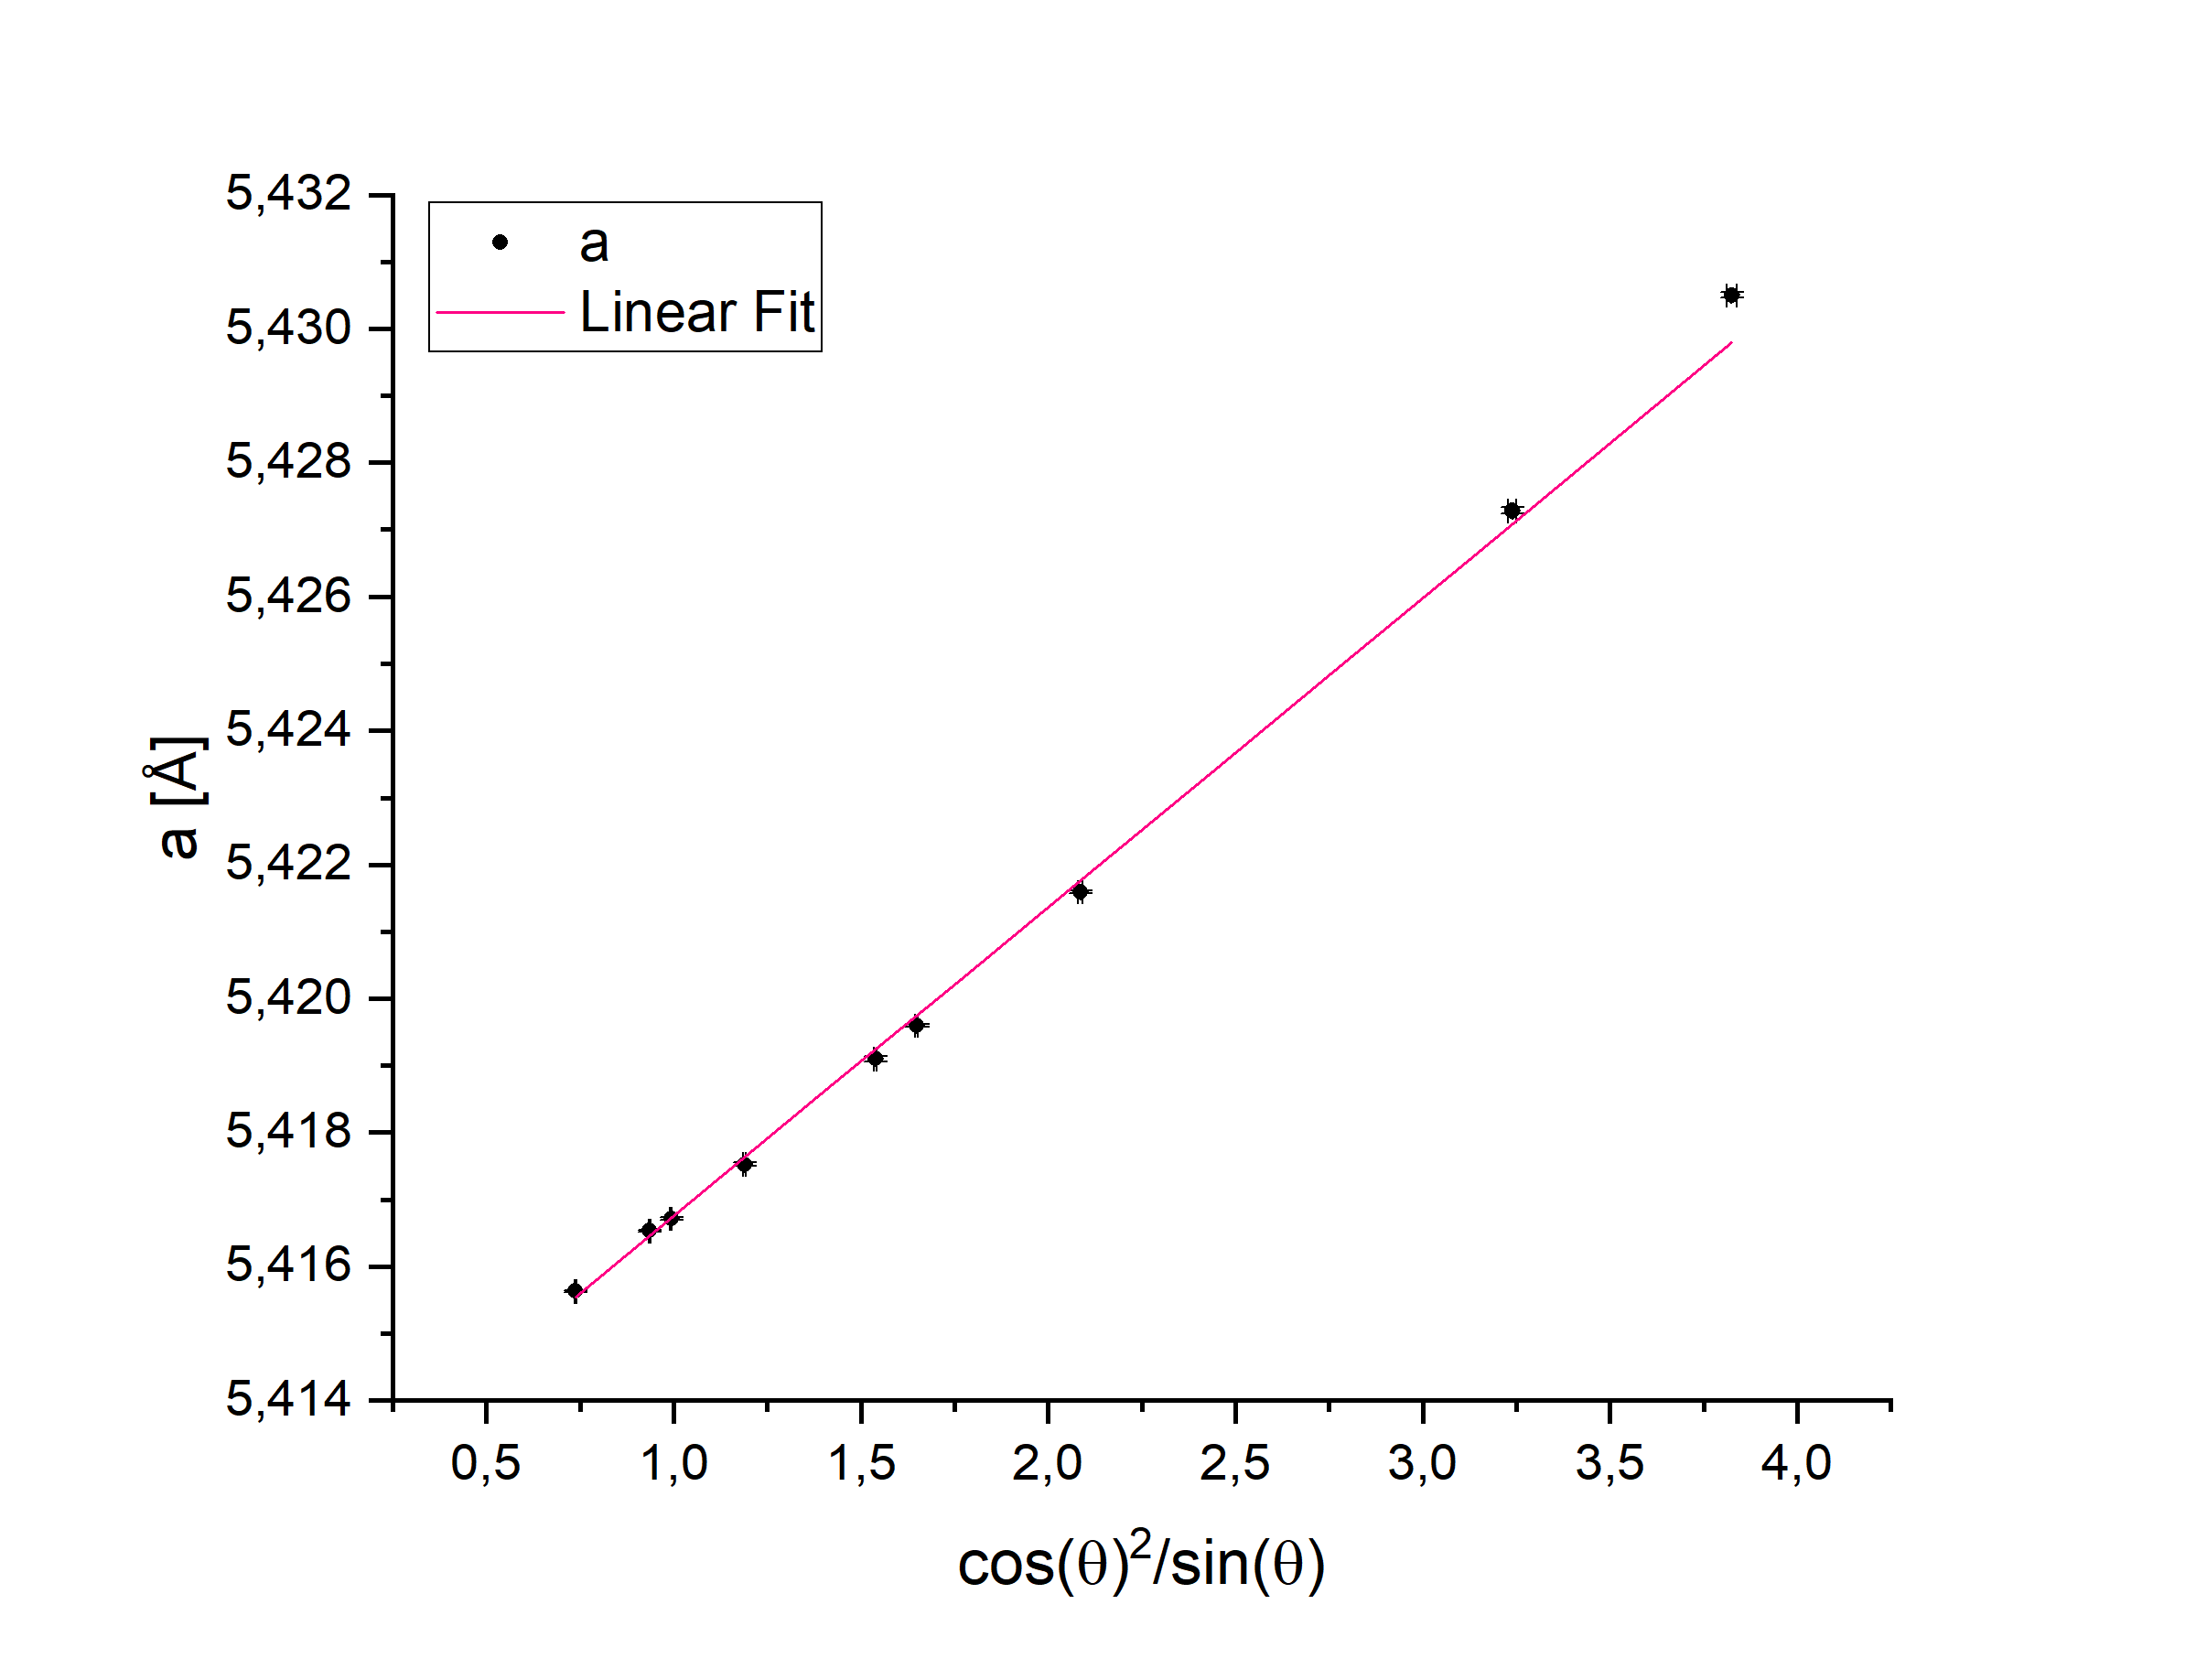
\includegraphics[width=0.7\textwidth]{2_XRD/Graphics/Experiments/Lattice Constants/LatticeConstant_CeO2_1.png}
    \caption{Plot of the lattice constant $a$ for micro-crystalline \ce{CeO2}}
    \label{fig:LatticeConstant_CeO2_1}
\end{figure}
\FloatBarrier

\begin{figure}[!ht]
    \centering
    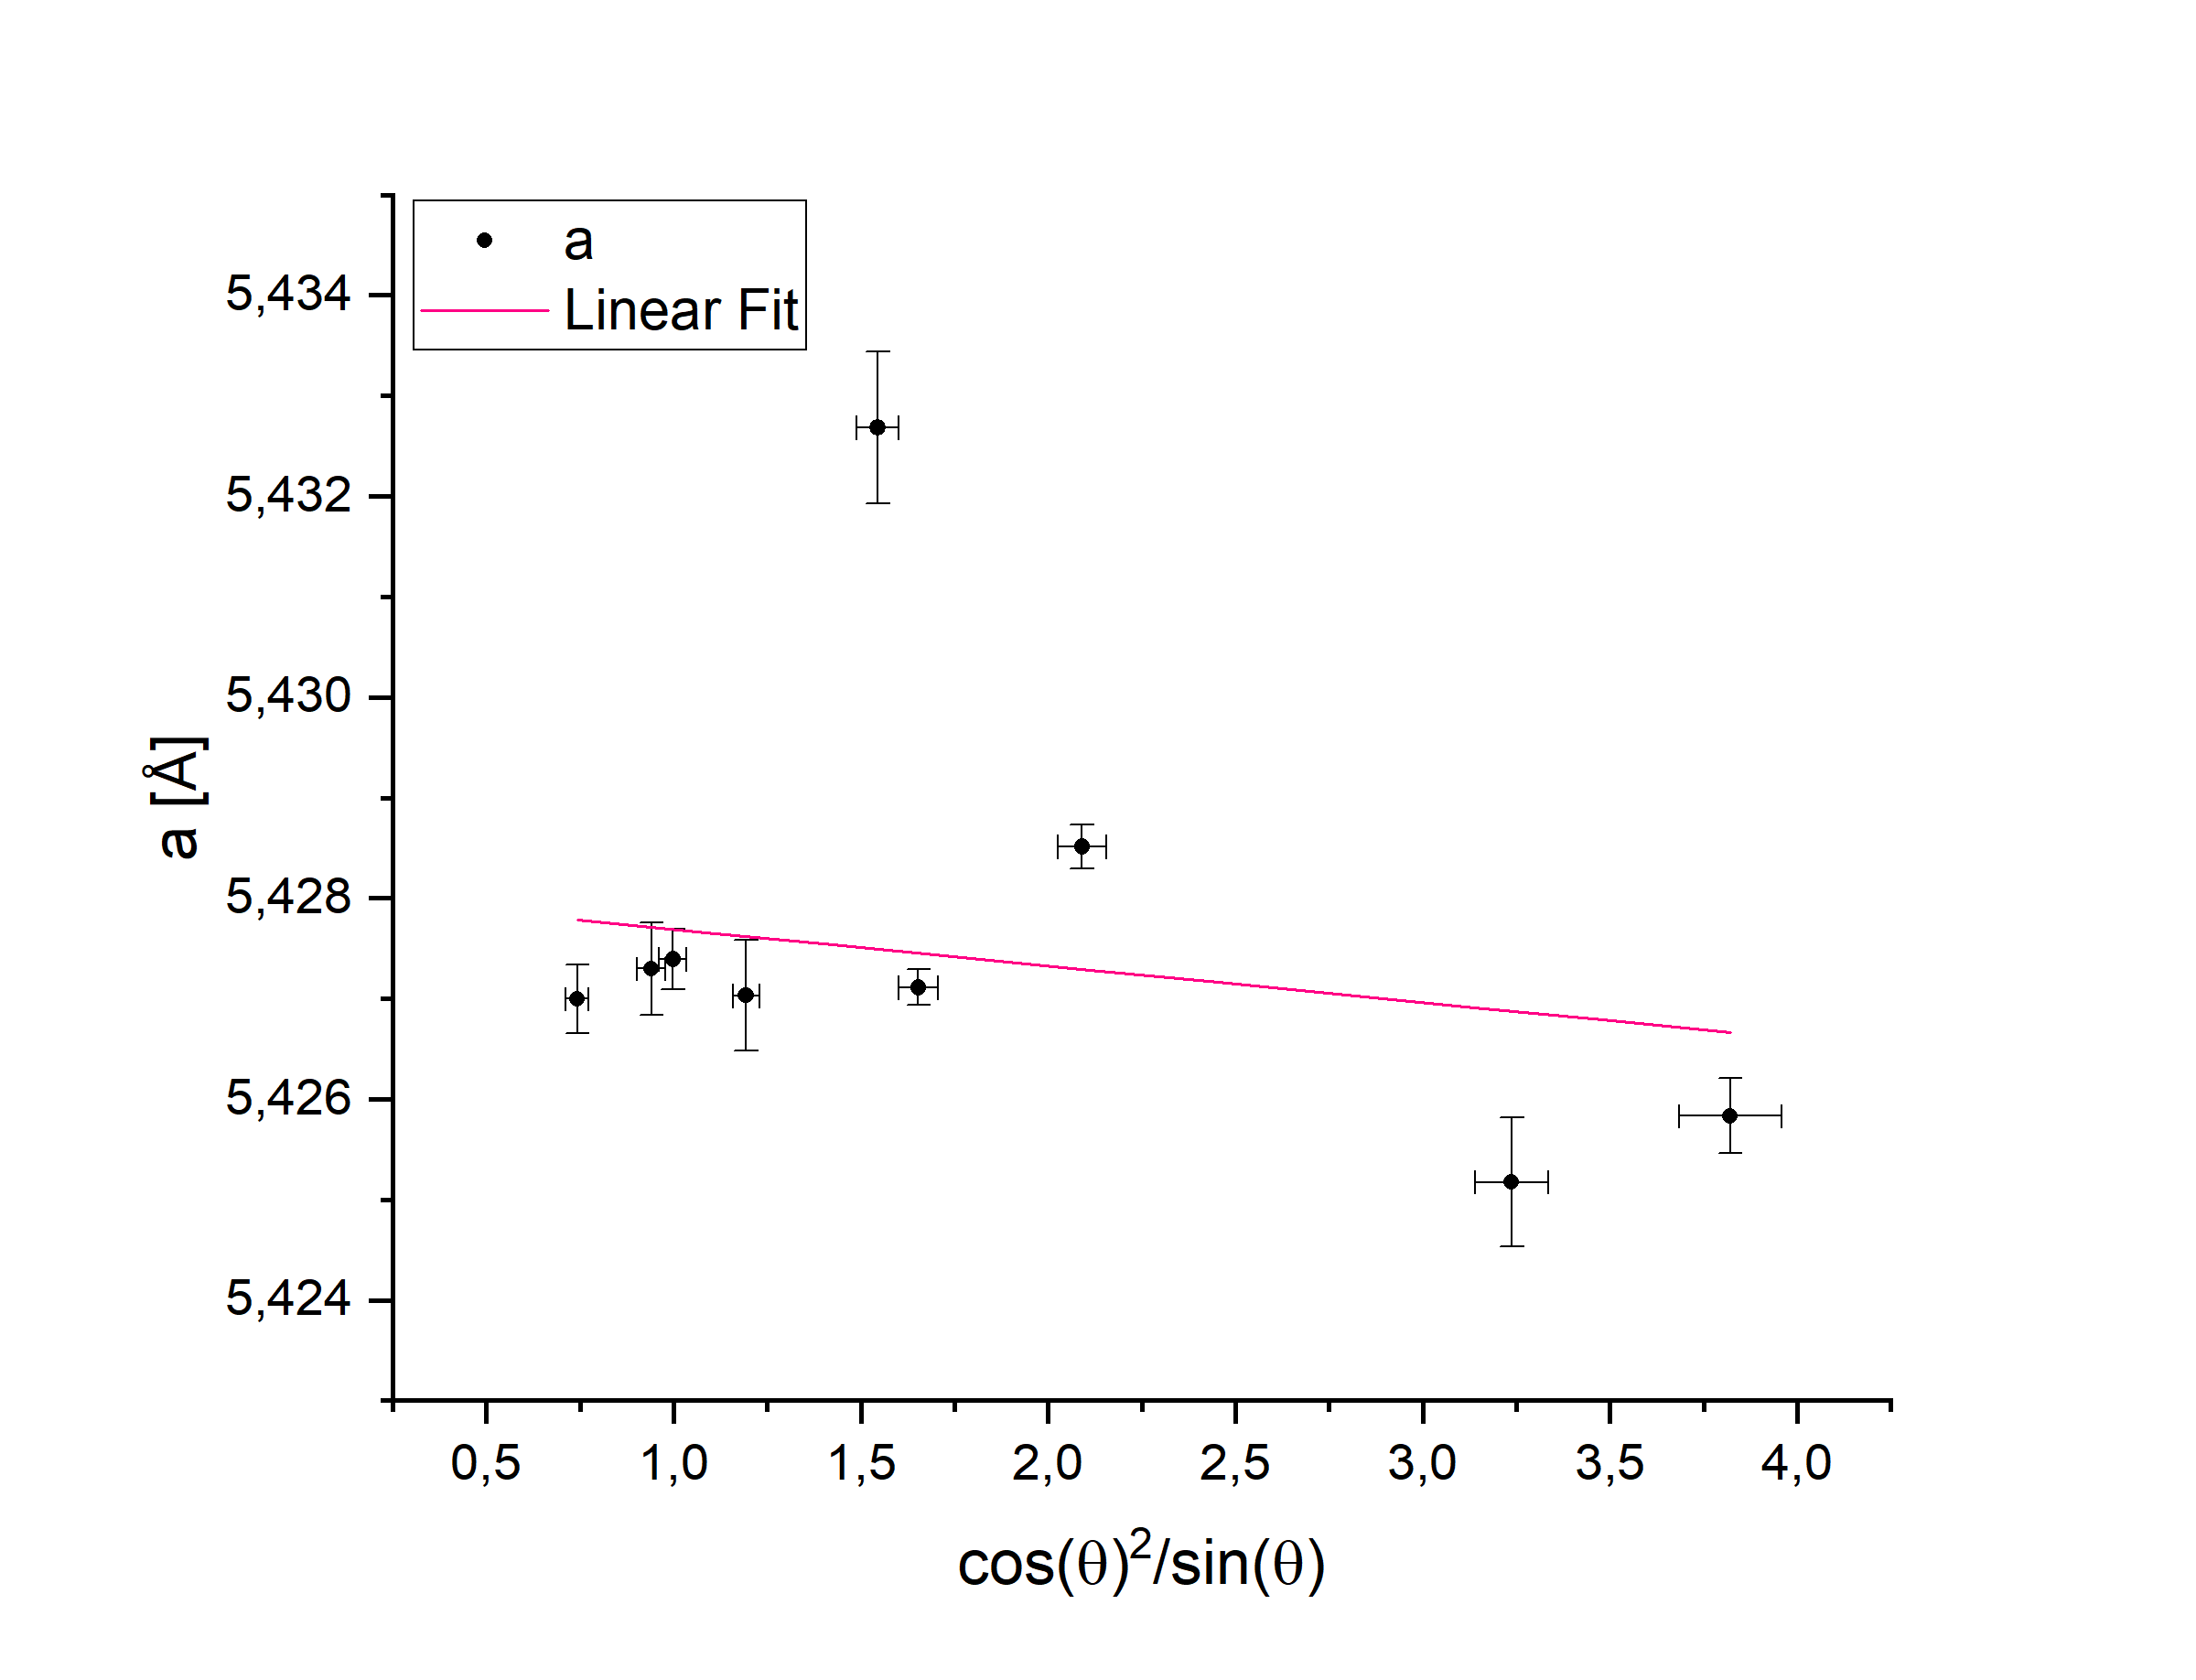
\includegraphics[width=0.7\textwidth]{2_XRD/Graphics/Experiments/Lattice Constants/LatticeConstant_CeO2_2.png}
    \caption{Plot of the lattice constant $a$ for nano-crystalline \ce{CeO2}}
    \label{fig:LatticeConstant_CeO2_2}
\end{figure}
\FloatBarrier

\begin{figure}[!ht]
    \centering
    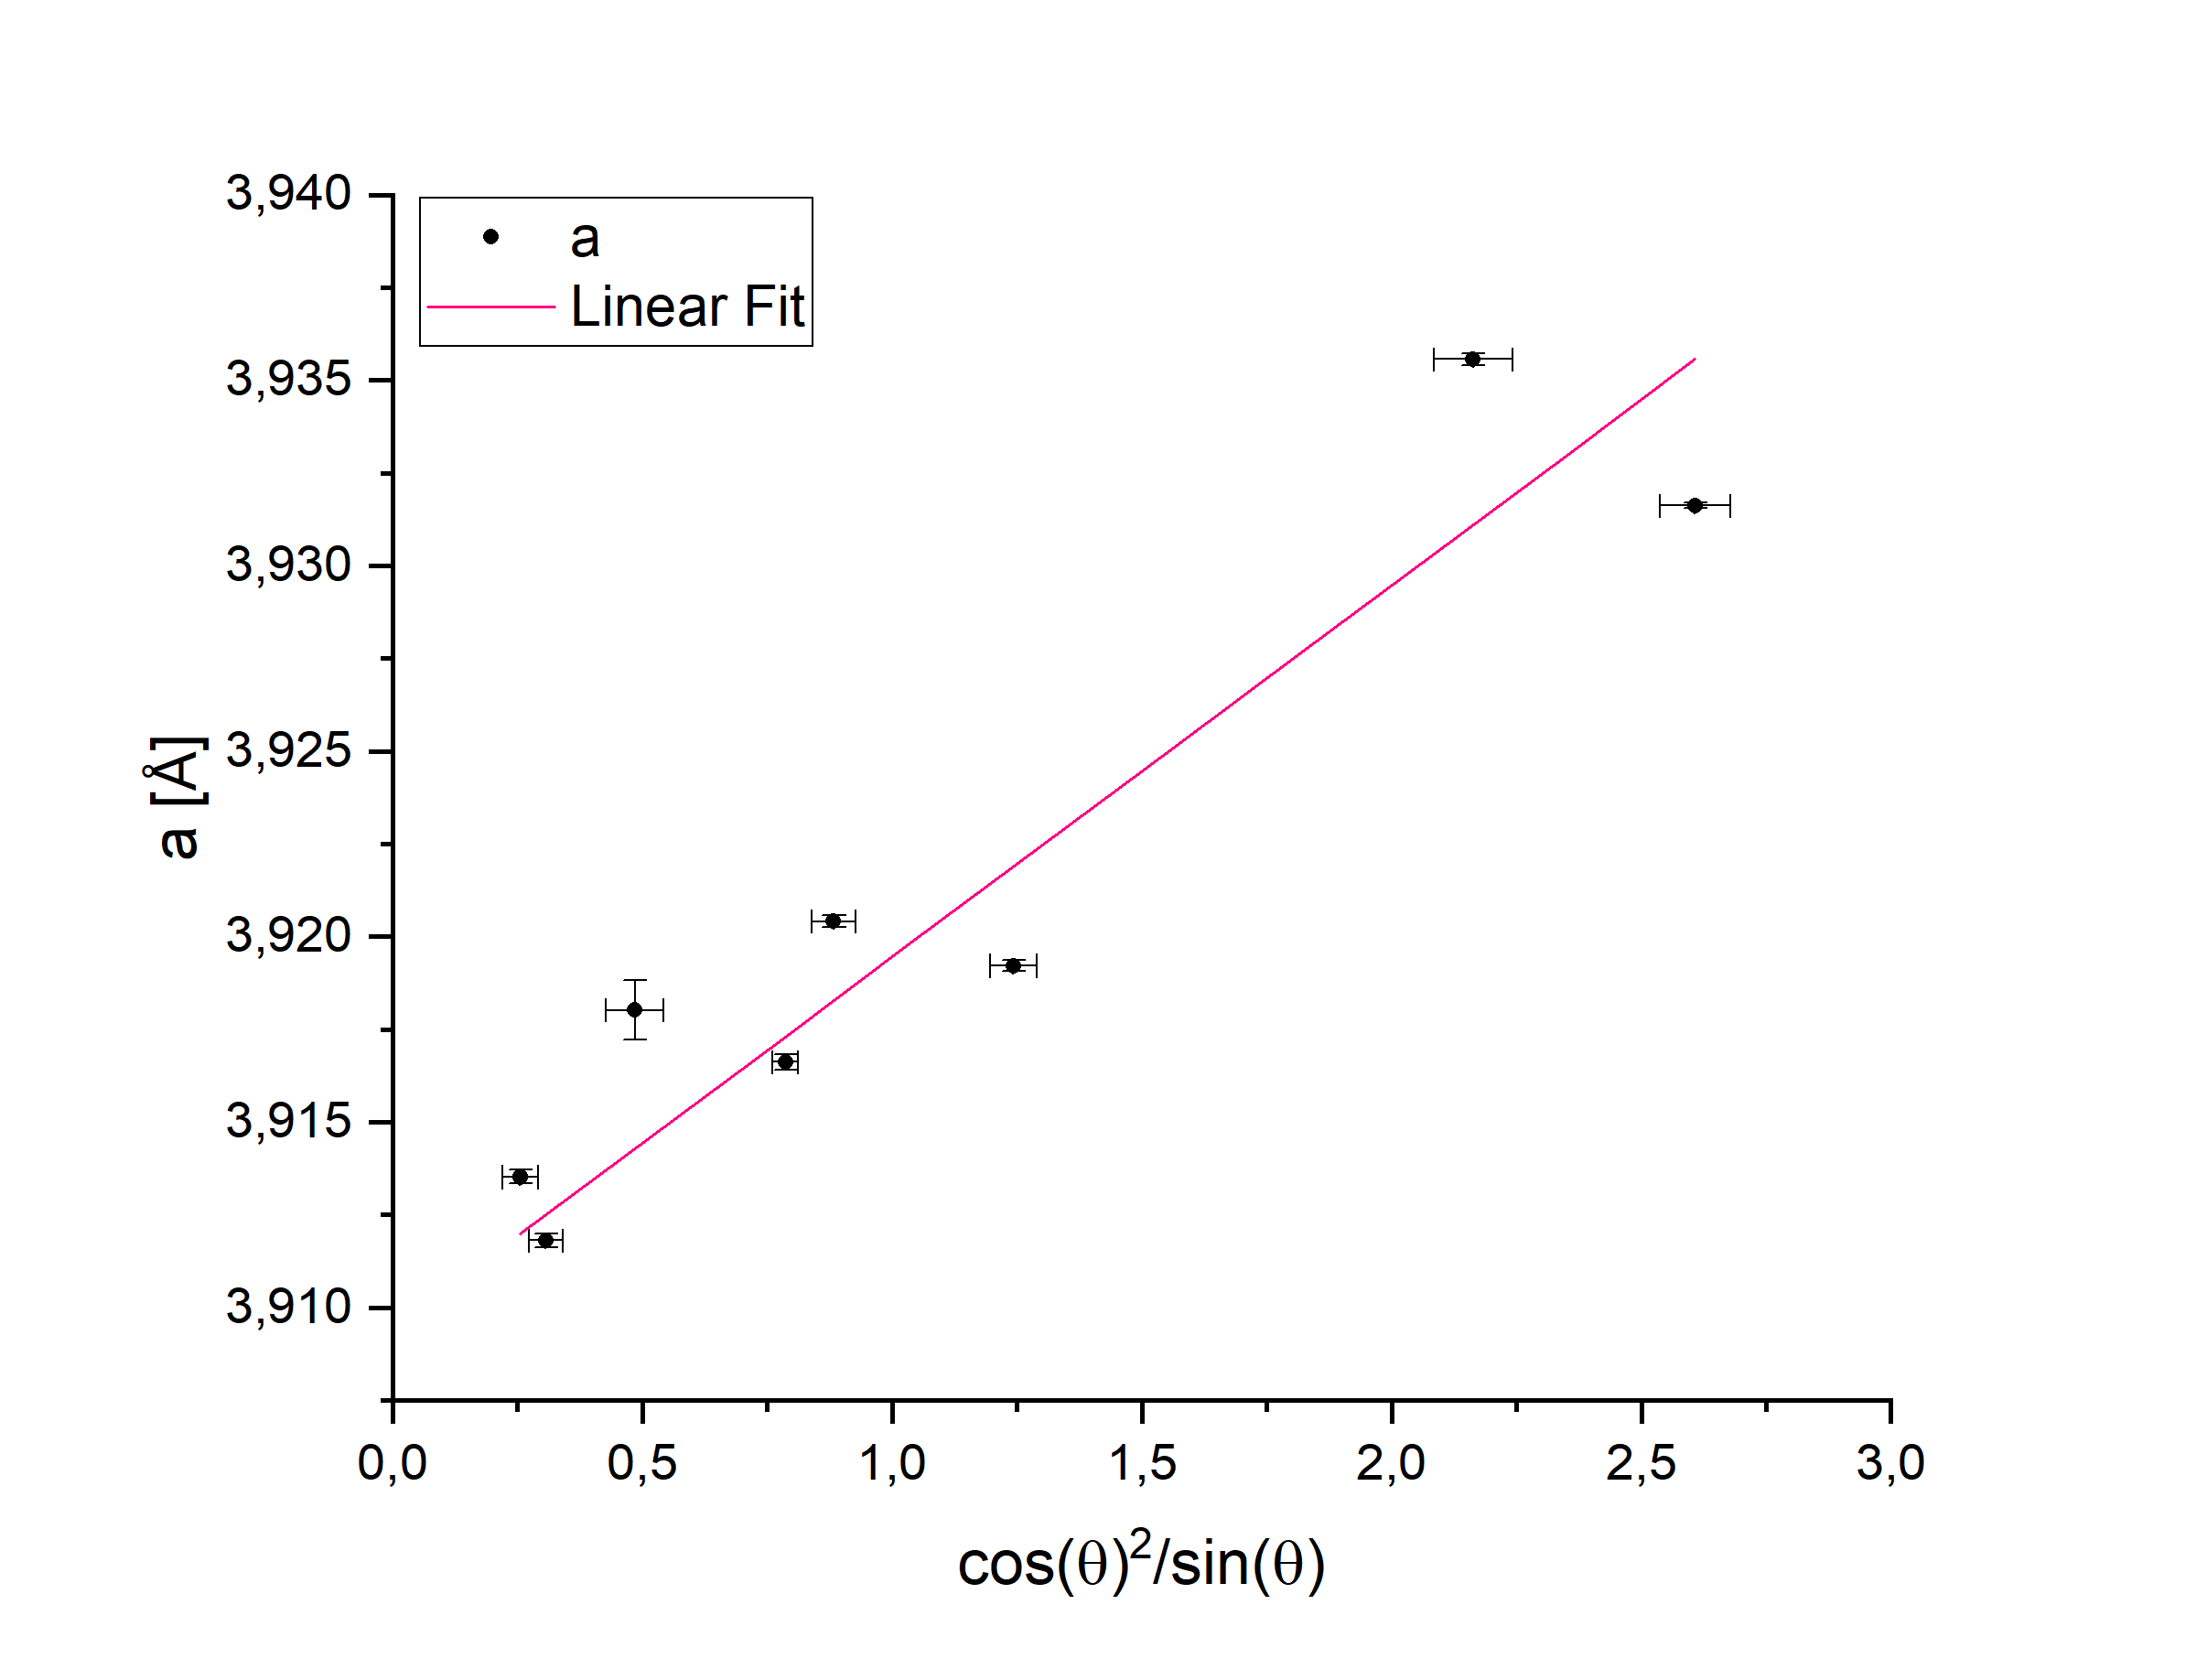
\includegraphics[width=0.7\textwidth]{2_XRD/Graphics/Experiments/Lattice Constants/LatticeConstant_Pd90Au10.png}
    \caption{Plot of the lattice constant $a$ for \ce{Pd90Au10}}
    \label{fig:LatticeConstant_Pd90Au10}
\end{figure}
\FloatBarrier

The resulting true lattice constants are the following:
\[
\begin{cases}
    a_0^{\ce{CeO2,1}} = (5,4122 \cdot 10^{-10} \pm 1,34329 \cdot 10^{-14}) \ \text{m} \\
    a_0^{\ce{CeO2,2}} = (5,42815 \cdot 10^{-10} \pm 9,65352 \cdot 10^{-14}) \ \text{m} \\
    a_0^{\ce{Pd90Au10}} = (3,91117 \cdot 10^{-10} \pm 2,17413 \cdot 10^{-13}) \ \text{m}
\end{cases}
\]

The experimentally determined value for \ce{CeO2} is matching the literature value of $a_{\ce{CeO2}} = 5,41 \cdot 10^{-10} \ \text{m}$ \cite{CeriumOxide}. It is noticeable, that the lattice constant for the micro-crystalline \ce{CeO2} is slightly smaller than for the nano-crystalline \ce{CeO2}. This is due to the crystals having a surface charge which leads to Coulomb interaction between crystals, resulting in slight variations in the crystallite size. \\

For a mixture of compounds, a good rule of thumb is Vegard's law: for two elements $X$ and $Y$ in proportions $x:(1-x)$, the resulting lattice constant is \cite{VegardLaw}:
\begin{equation}
    a_{XY} = (1-x)a_X + xa_Y
\end{equation}

Using the literature values for $a_{Pd}$ and $a_{Au}$ \cite{LatticeCsts}, we can compute the expected $a_{\ce{Pd90Au10}}$ as:
\begin{equation}
    a_{\ce{Pd90Au10}} = 0,9 \cdot a_{Pd} + 0,1 \cdot a_{Au} 
\end{equation}

Which yields $a_{\ce{Pd90Au10}} = 3,88 \cdot 10^{-10} \ \text{m}$, and matches the experimentally determined value. \\

\subsection{Instrumental Broadening}
In order to remove the broadening due to the instruments, we use the \ce{LaB6} sample. It is in powder form, with very different crystallite sizes, thus eliminating their influence on the broadening. The preparation process is such that there is little to no strain. The resulting total broadening is then due to instrumental sources only.
We fit the Caglioti function 
\begin{equation}
    f(\theta) = \sqrt{A + B \tan(\theta) + C \tan^2(\theta)}
\end{equation}
onto the data from the \ce{LaB6} sample (see fig. \ref{fig:CagliotiFit}).

We can later subtract $f(\theta)$ from the total broadening to remove the instrumental broadening.

\begin{figure}[!ht]
    \centering
    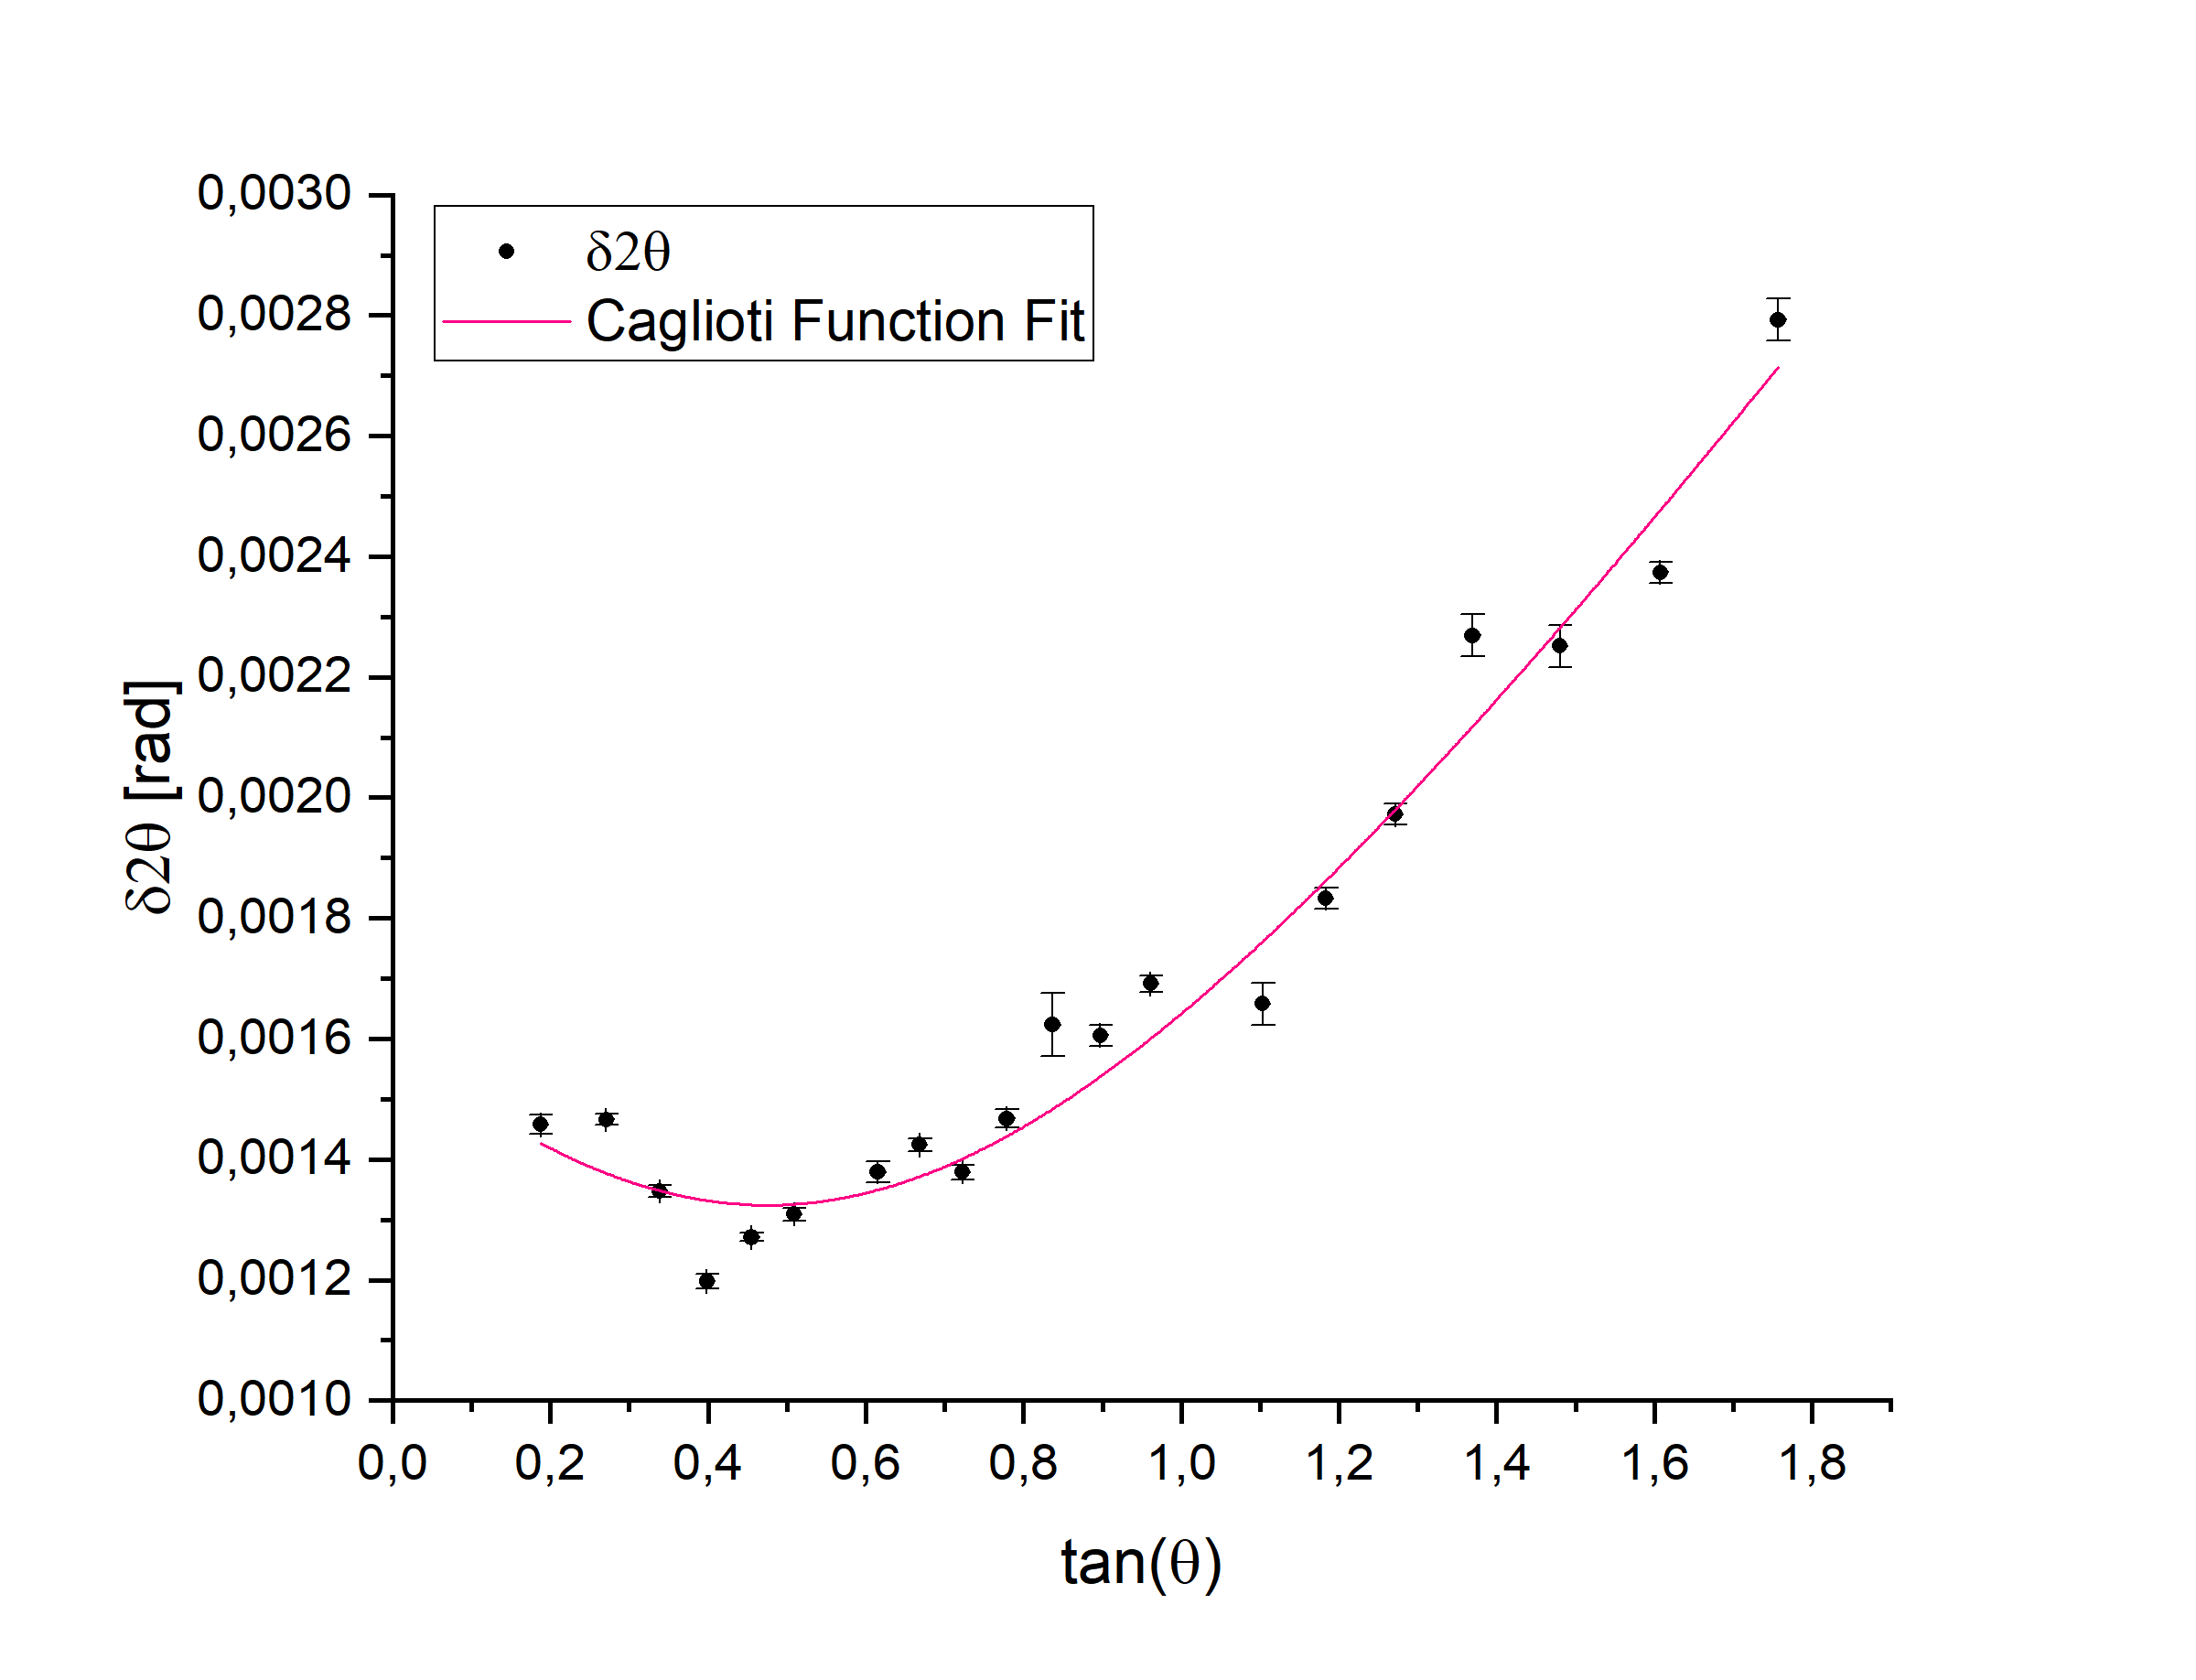
\includegraphics[width=0.8\textwidth]{2_XRD/Graphics/Experiments/Instrumental Broadening/CagliotiFit.png}
    \caption{Plot of the FWHM of \ce{LaB6}, fitted with the Caglioti function}
    \label{fig:CagliotiFit}
\end{figure}
\FloatBarrier

From the fit we obtain the following values of $A,B,C$:
\[ 
\begin{cases}
    A = ( 2,52585 \pm 0,201128 ) \cdot 10^{-6} \ \text{rad}^2 \\
    B = (-3,25011 \pm 0,603034 ) \cdot 10^{-6} \ \text{rad}^2 \\
    C = ( 3,41849 \pm 0,384497 ) \cdot 10^{-6} \ \text{rad}^2
\end{cases}
\]




\subsection{Strain and crystallite size}

In this section we will use two approaches to determine the  strain in the crystal and the average crystallite size. The idea is to either approximate the peaks as Lorentzian-shaped peaks or as Gaussian-shaped peaks.   

We first perform the change of variable to $s$ and $\delta s$. Then we apply linear fits to determine the strain $e$ and crystallite sizes $D$ using eq. \ref{eq:LorentzianStrainSize} and eq. \ref{eq:GaussianStrainSize}. The slopes and intercepts at origin then give us the values of $e$ and $D$. The data points are scattered a lot around the linear fit due to anisotropic elasticity. The elastic modulus changes depending on the orientation of the crystal in relation to the incoming beam, thus resulting in tiny changes in the computed crystallite size and strain. This effect is however not taken into account for our calculations, as we estimate it is getting averaged out over the data range.

\subsubsection{Lorentzian Approach}

\begin{figure}[!ht]
    \begin{subfigure}{0.5\textwidth}
        \centering
        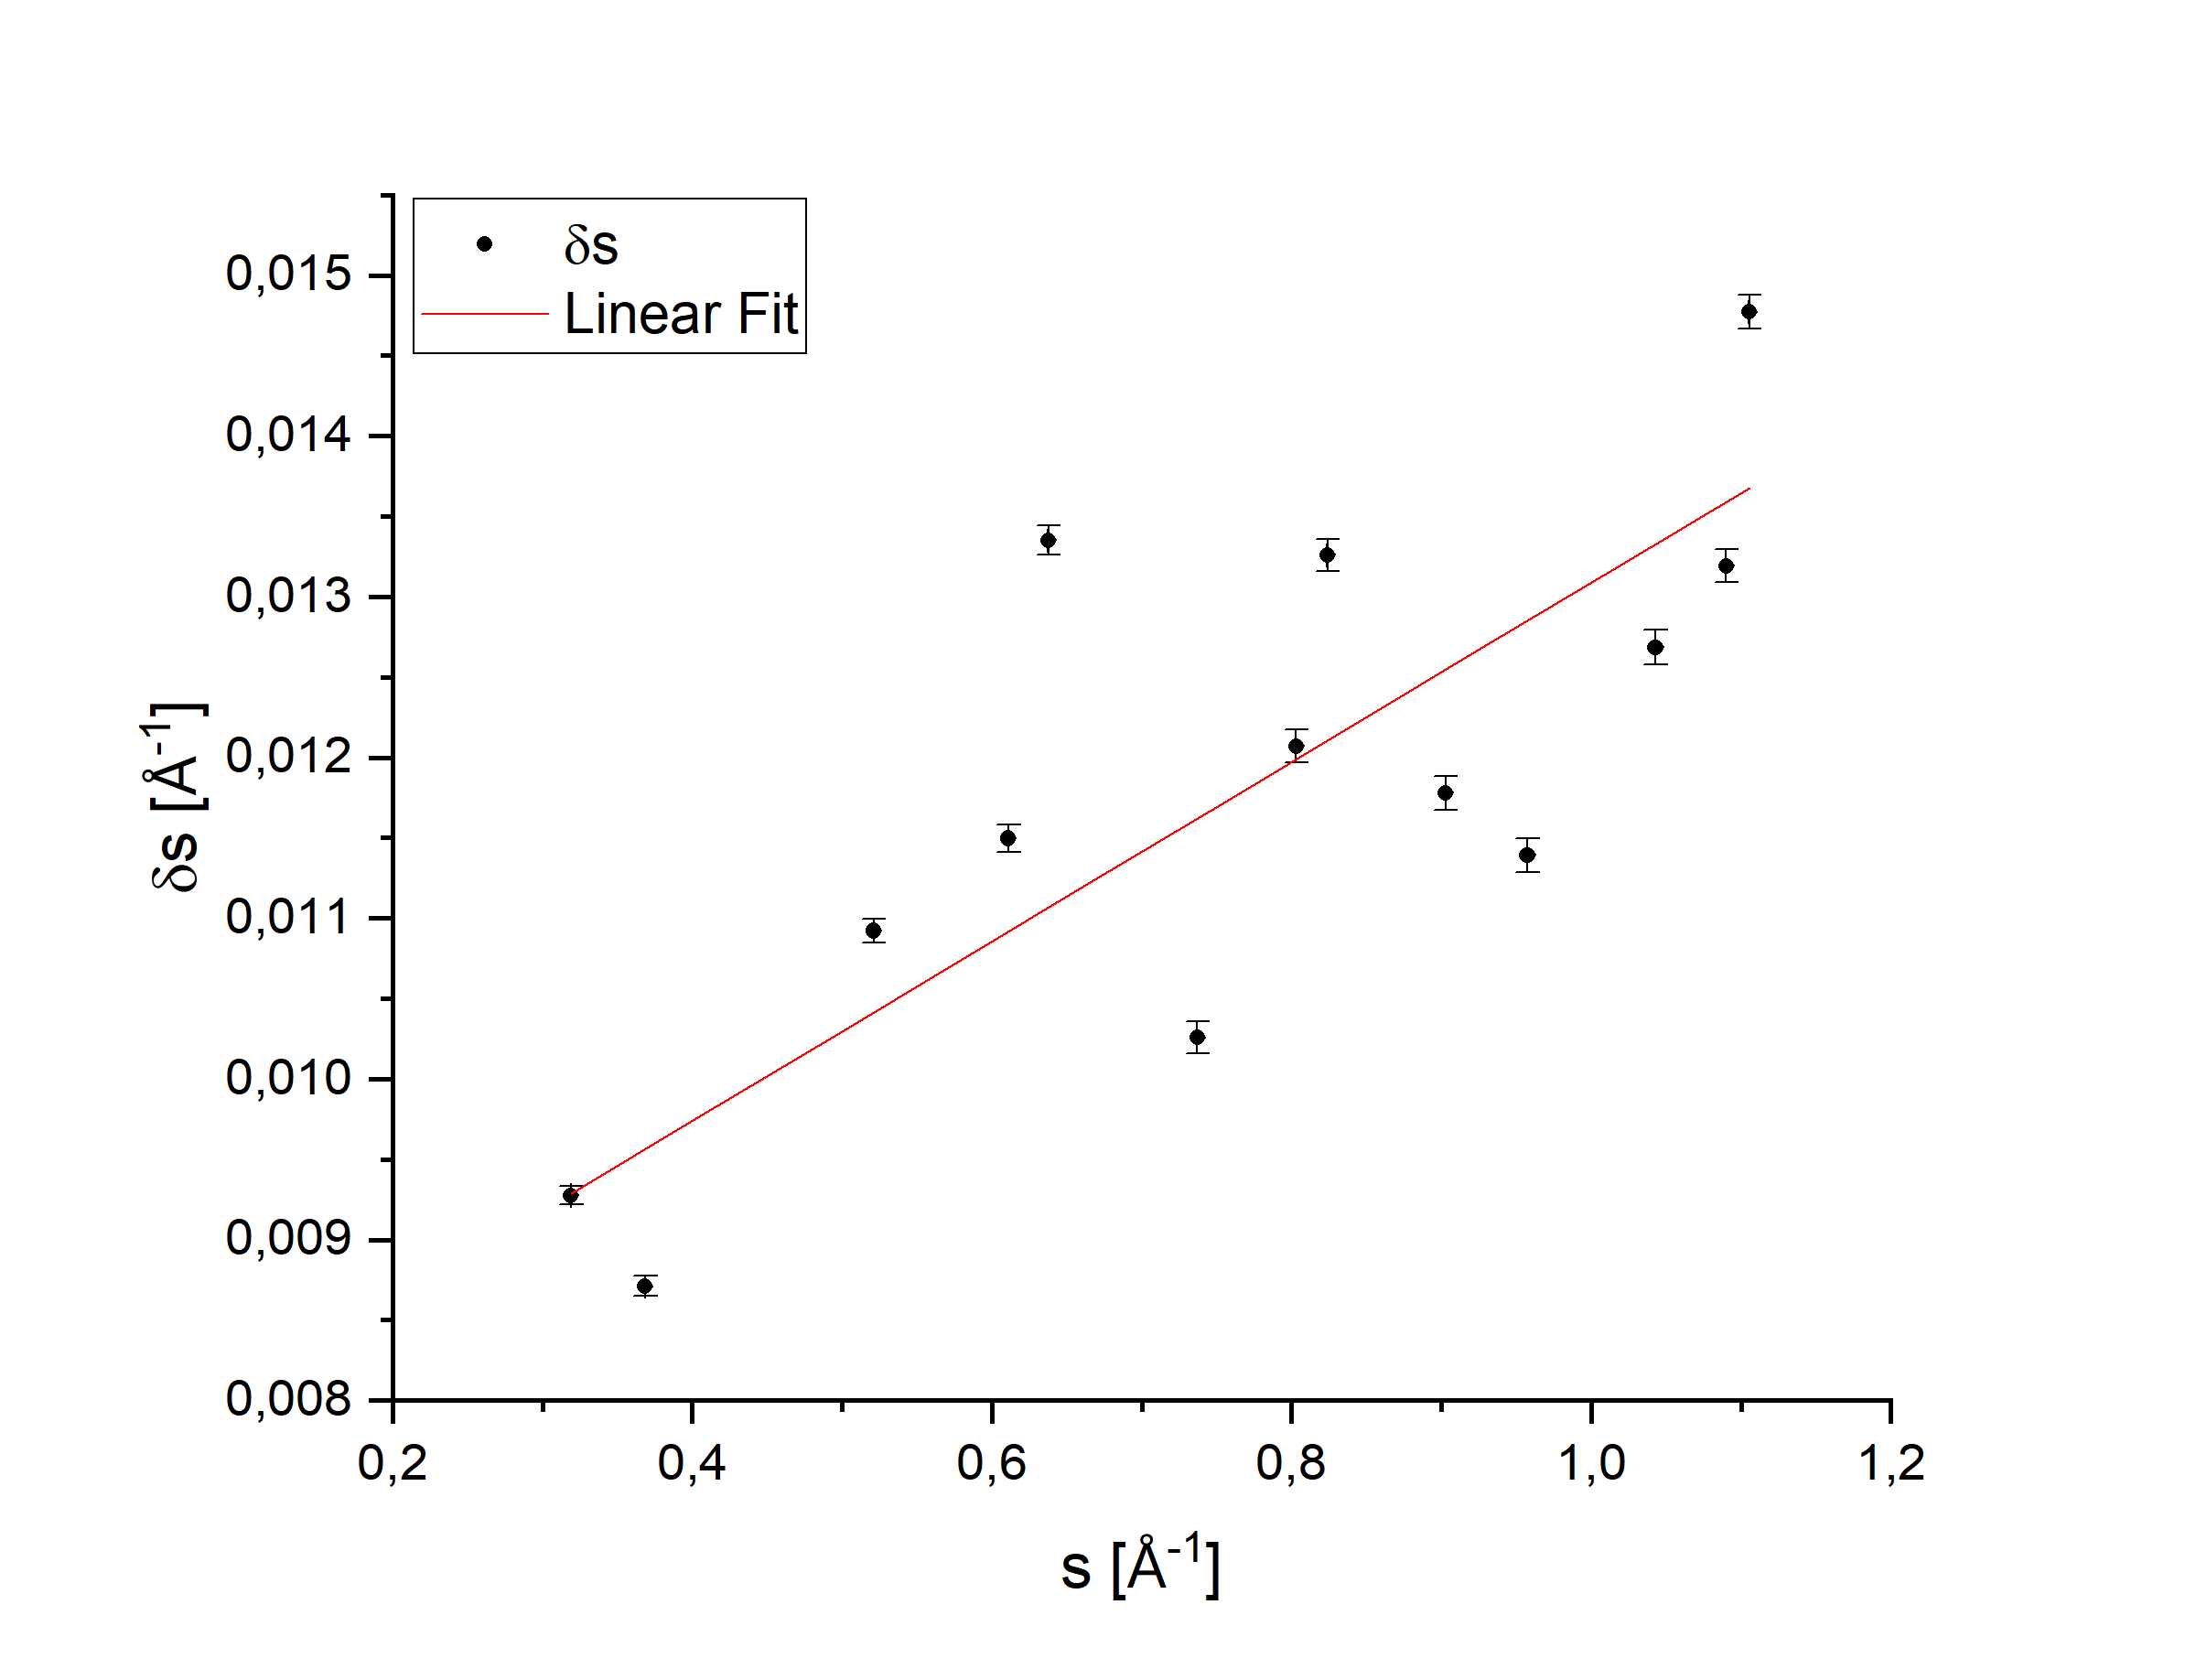
\includegraphics[width=\textwidth]{2_XRD/Graphics/Experiments/Lorentzian Broadening/LorentzianBroadening_CeO2_2.png}
        \caption{nano-crystalline \ce{CeO2}}
    \end{subfigure}
    \begin{subfigure}{0.5\textwidth}
        \centering
        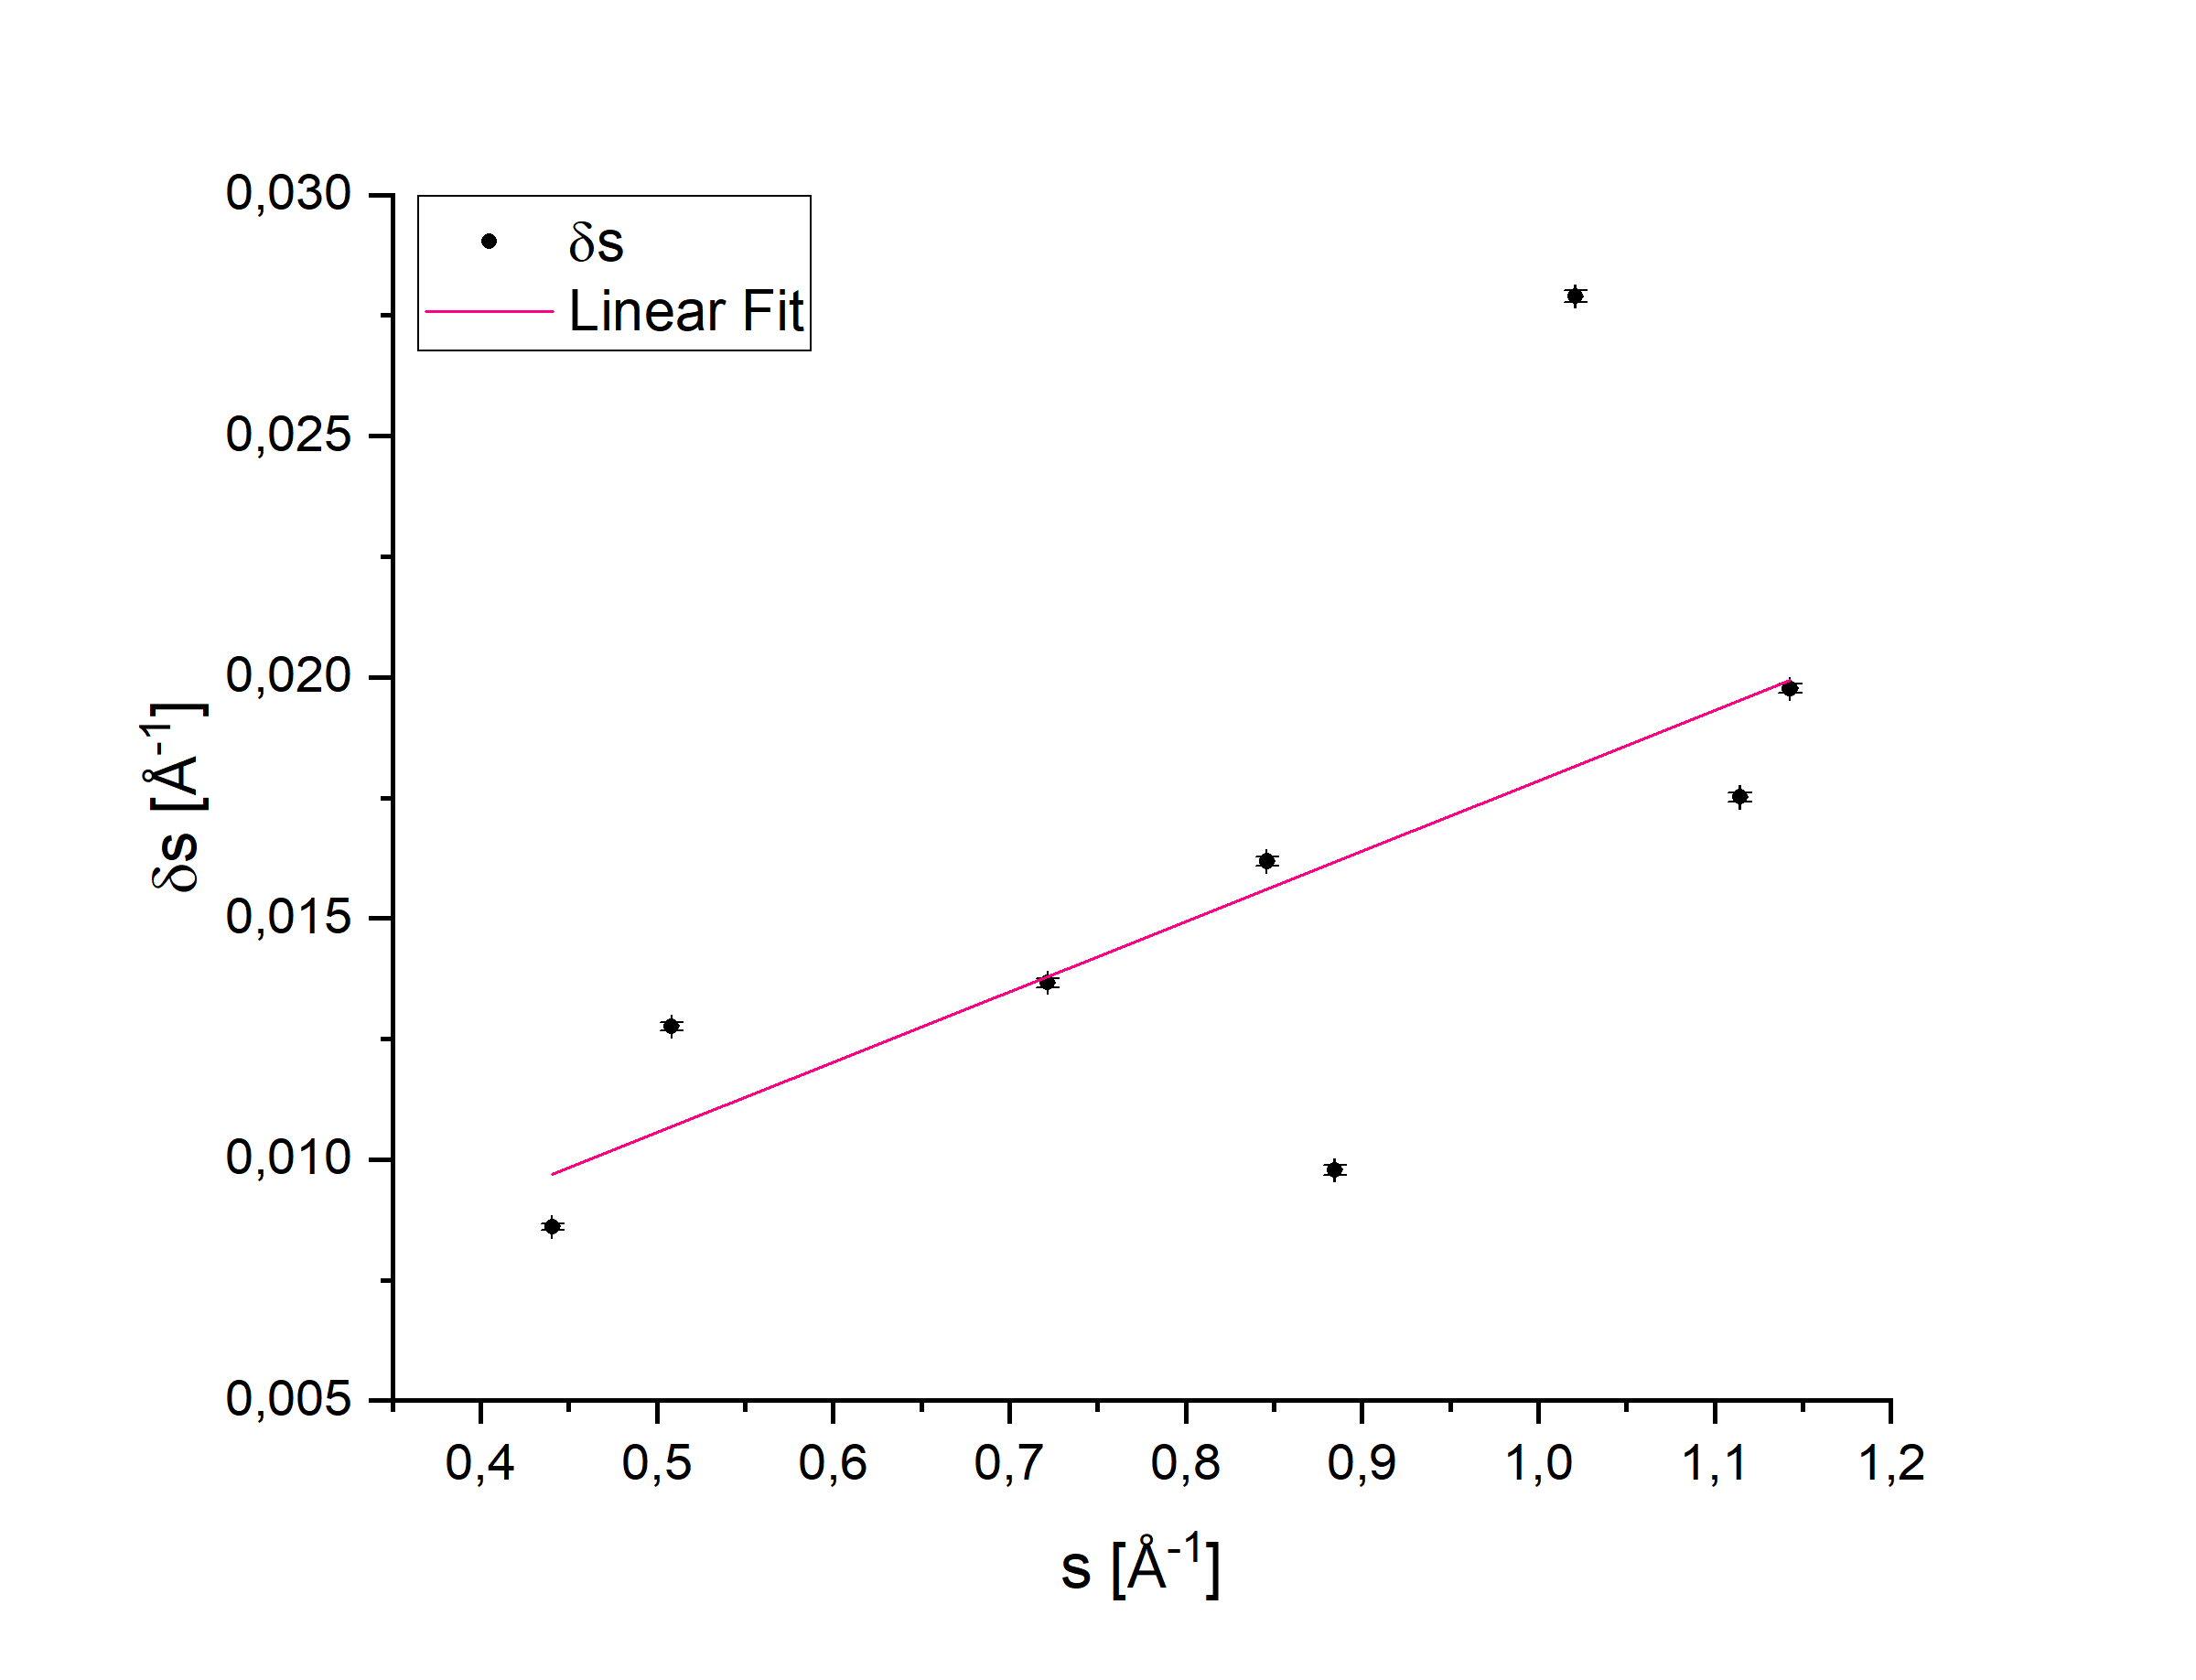
\includegraphics[width=\textwidth]{2_XRD/Graphics/Experiments/Lorentzian Broadening/LorentzianBroadening_Pd90Au10.png}
        \caption{\ce{Pd90Au10}}
    \end{subfigure}
    \caption{Plots of $\delta s$ against $s$ with a Lorentzian profile approach}
    \label{fig:LorentzianStrainSize}
\end{figure}
\FloatBarrier

The linear fit equations are of the form $y = mx+p$, yielding for \ce{CeO2}:
\[
\begin{cases}
    m = (5,43 \pm 0,98) \cdot 10^{-3}  \\
    p = (7,62 \pm 0,60) \cdot 10^{-3} \textup{~\AA}^{-1}
\end{cases}
\]
and for \ce{Pd90Au10}:
\[
\begin{cases}
    m = (14,02 \pm 3,09) \cdot 10^{-3} \\
    p = (3,23 \pm 2,10) \cdot 10^{-3} \textup{~\AA}^{-1}
\end{cases}
\]

Using eq. \ref{eq:LorentzianStrainSize}, we obtain the following values for strain and crystallite size for \ce{CeO2}:
\[
\begin{cases}
    D_L^{\ce{CeO2}} = (15,75 \pm 1,23) \ \text{nm}\\
    e_L^{\ce{CeO2}} = (0,27 \pm 0,05) \ \%
\end{cases}
\]

And for \ce{Pd90Au10} we get:
\[
\begin{cases}
    D_L^{\ce{Pd90Au10}} = (37,15 \pm 24,15) \ \text{nm}\\
    e_L^{\ce{Pd90Au10}} = (0,70 \pm 0,16) \ \%
\end{cases}
\]

\newpage
\subsubsection{Gaussian Approach}

\begin{figure}[!ht]
    \begin{subfigure}{0.5\textwidth}
        \centering
        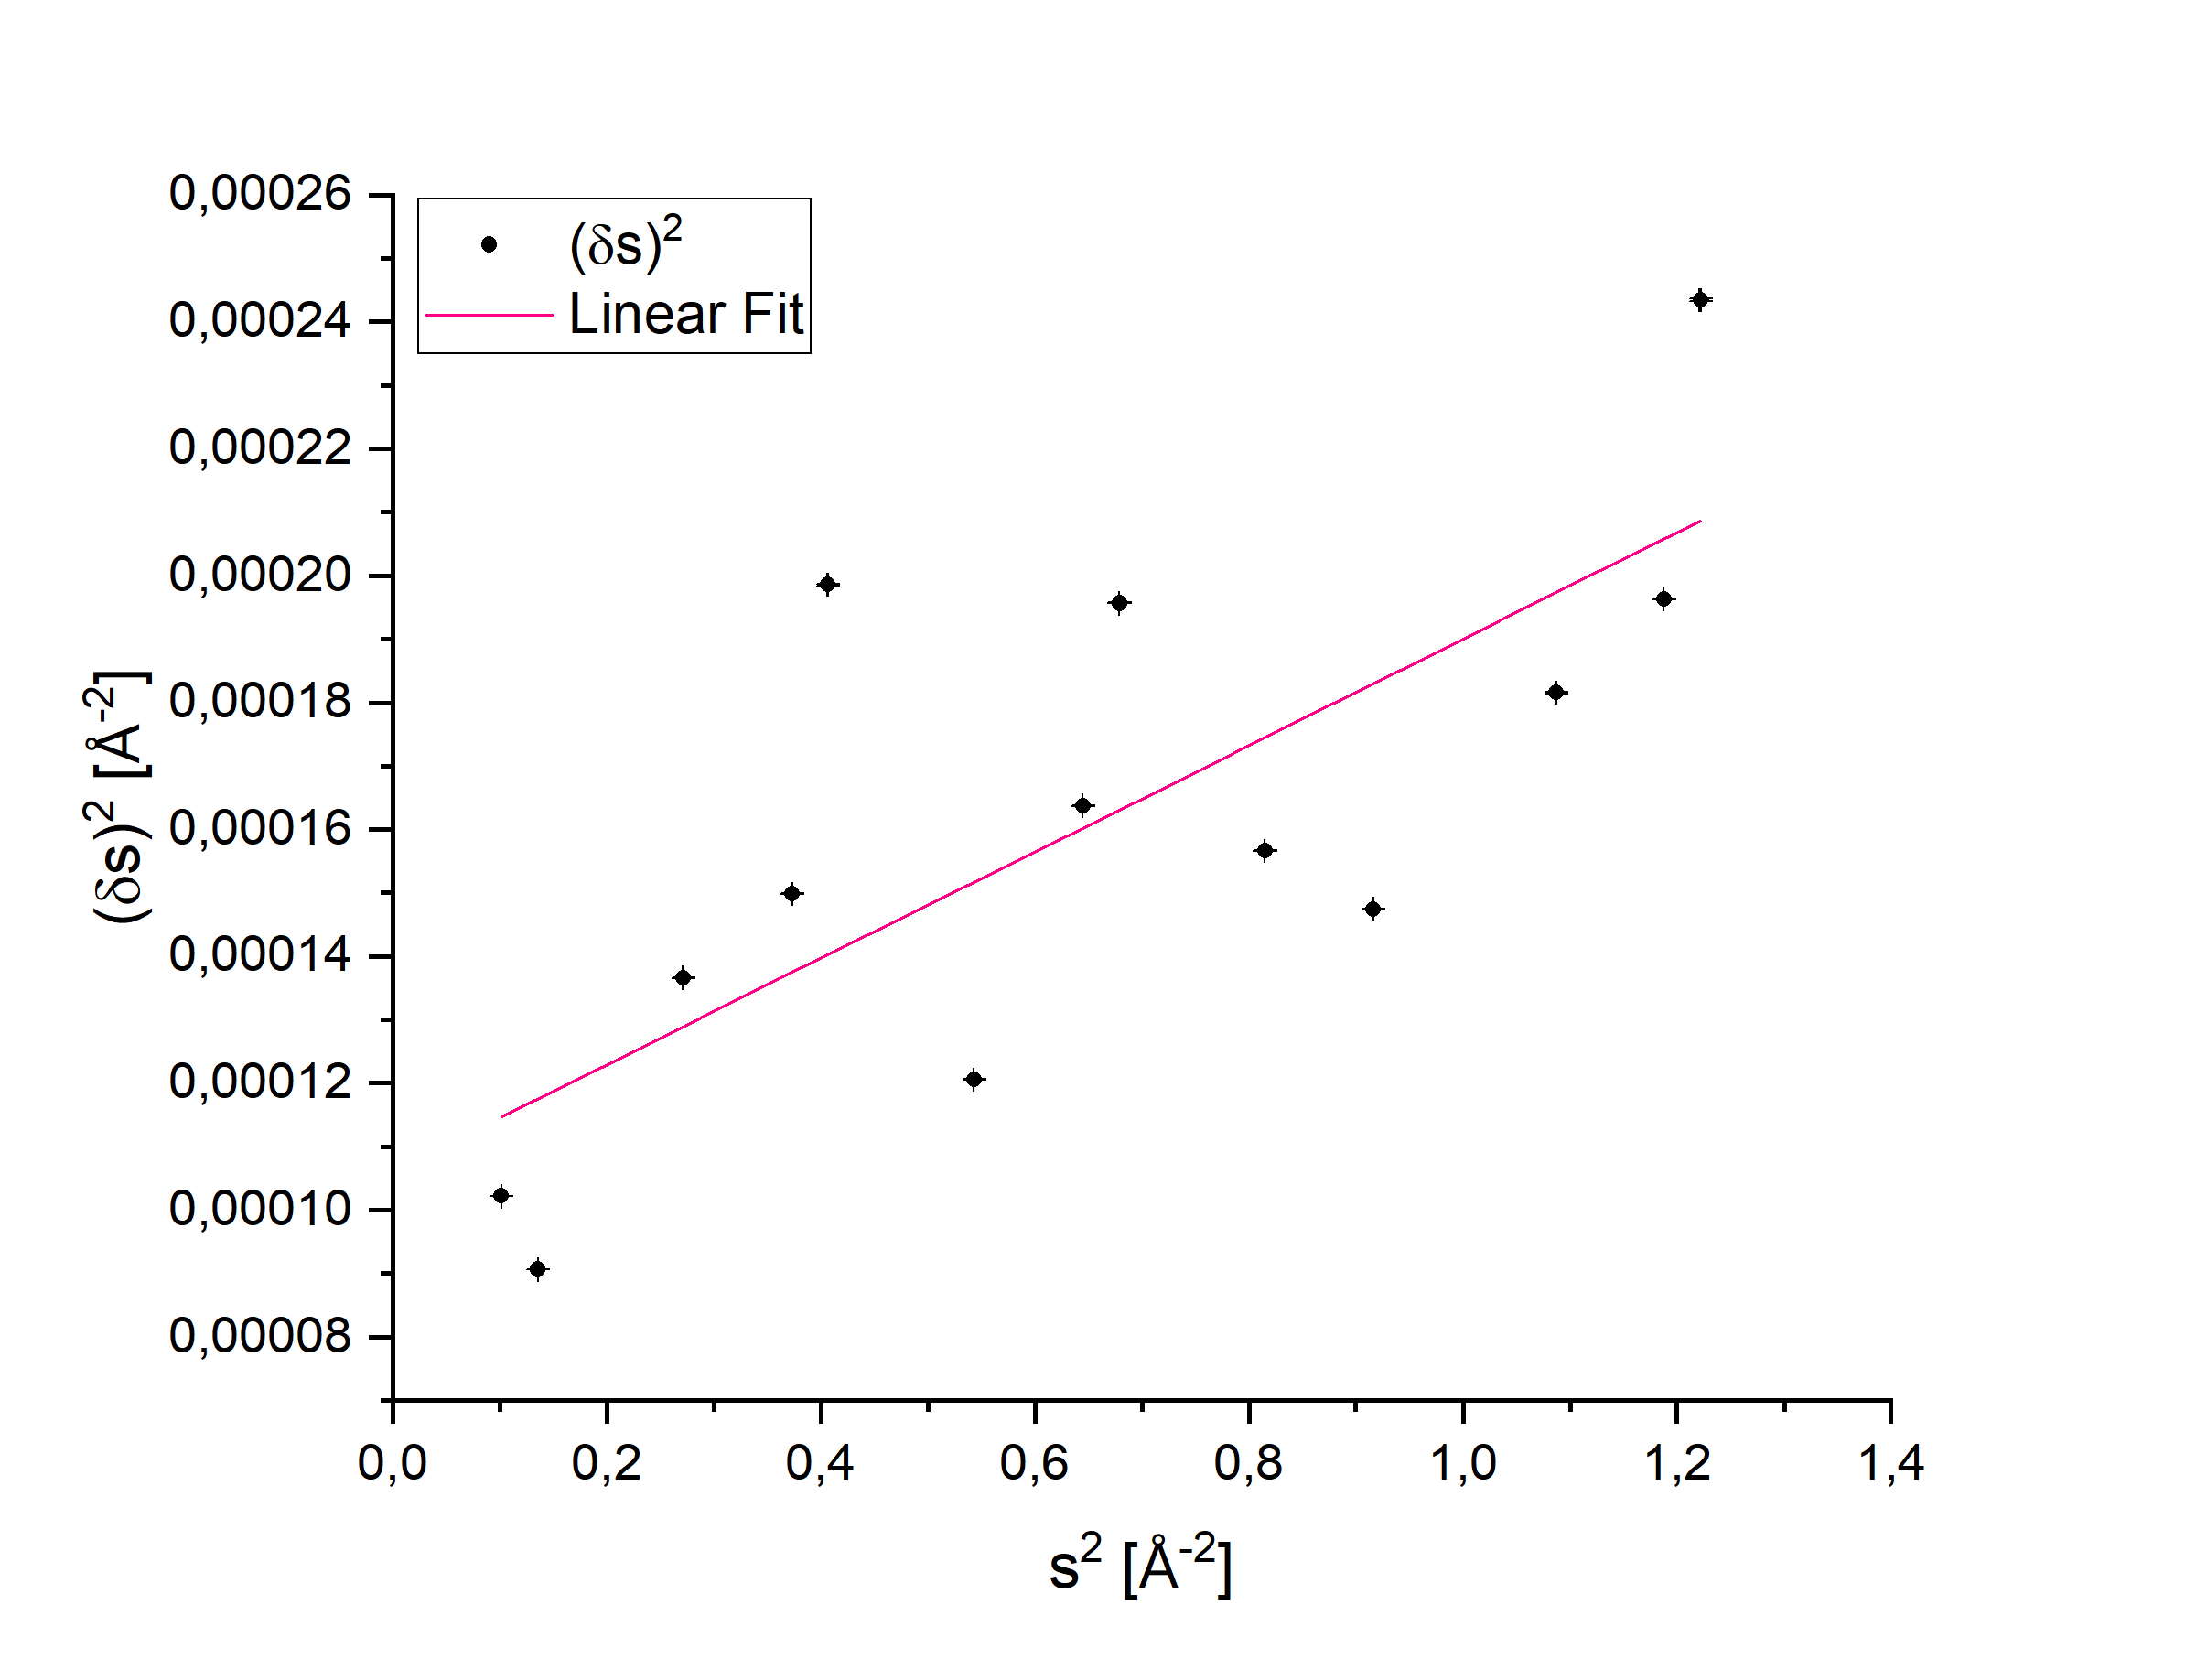
\includegraphics[width=\textwidth]{2_XRD/Graphics/Experiments/Gaussian Broadening/GaussianBroadening_CeO2_2.png}
        \caption{nano-crystalline \ce{CeO2}}
    \end{subfigure}
    \begin{subfigure}{0.5\textwidth}
        \centering
        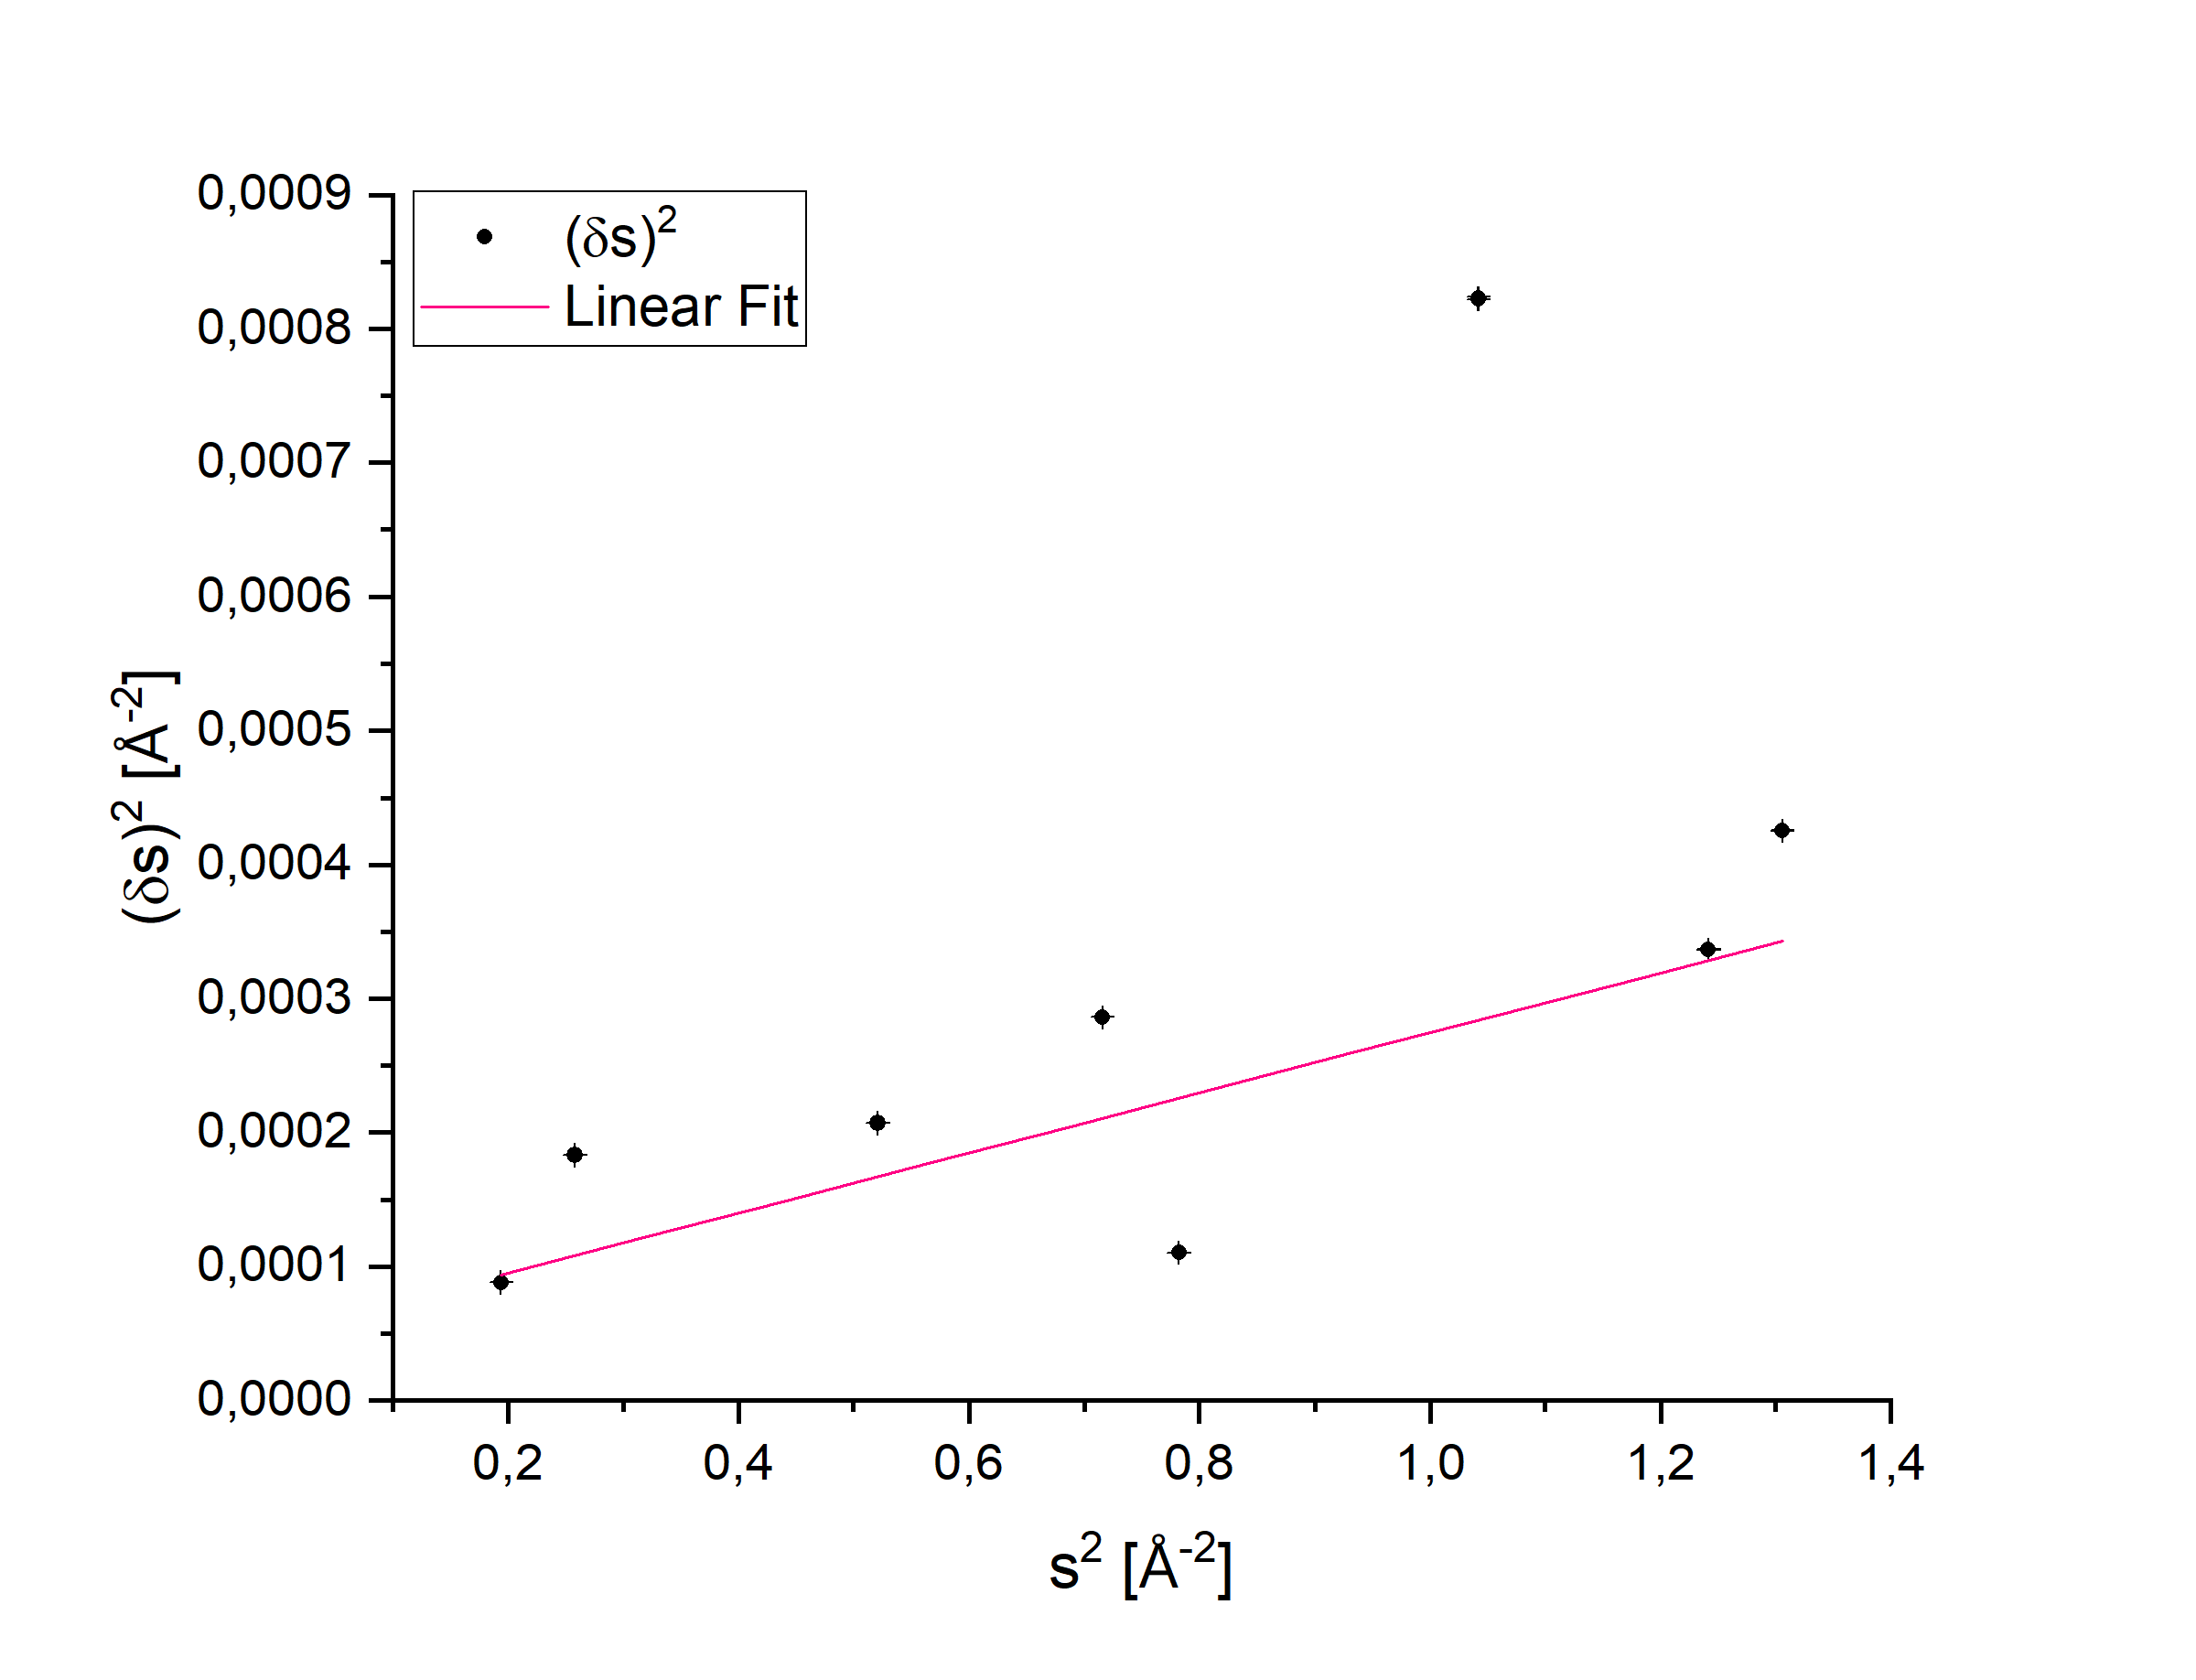
\includegraphics[width=\textwidth]{2_XRD/Graphics/Experiments/Gaussian Broadening/GaussianBroadening_Pd90Au10.png}
        \caption{\ce{Pd90Au10}}
    \end{subfigure}
    \caption{Plots of $(\delta s)^2$ against $s^2$ with a Gaussian profile approach}
    \label{fig:GaussianStrainSize}
\end{figure}
\FloatBarrier

The linear fit equations are of the form $y = mx+p$, yielding for \ce{CeO2}:
\[
\begin{cases}
    m = (9,53998 \pm 2,02715) \cdot 10^{-5} \\
    p = (9,31906 \pm 0,730979) \cdot 10^{-5} \textup{~\AA}^{-2}
    
\end{cases}
\]
and for \ce{Pd90Au10}:
\[
\begin{cases}
    m = (22,3453 \pm 7,75502) \cdot 10^{-5} \\
    p = (5,04927 \pm 2,44528) \cdot 10^{-5} \textup{~\AA}^{-2}
\end{cases}
\]

Using eq. \ref{eq:GaussianStrainSize}, we obtain the following values for strain and crystallite size for \ce{CeO2}:
\[
\begin{cases}
    D_G^{\ce{CeO2}} = (12,43 \pm 0,98) \ \text{nm}\\
    e_G^{\ce{CeO2}} = (0,49 \pm 0,05) \ \%
\end{cases}
\]

And for \ce{Pd90Au10} we get:
\[
\begin{cases}
    D_G^{\ce{Pd90Au10}} = (16,89 \pm 8,18)\ \text{nm}\\
    e_G^{\ce{Pd90Au10}} = (0,75 \pm 0,13) \ \%
\end{cases}
\]

\newpage

\section{Solved Problems}

\subsection{Problem 1}
\textbf{a)} Let $\{\Vec{a}_i\}$ and $\{\Vec{g}_i\}$ be the bases of the direct and reciprocal lattice respectively. The following relationship holds: $\Vec{g}_i \cdot \Vec{a}_j = 2\pi \delta_{ij}$.

The $(h,k,l)$ plane in the direct space can be described using three points in the direct space: $(\frac{1}{h} \Vec{a}_1, \frac{1}{k} \Vec{a}_2, \frac{1}{l} \Vec{a}_3)$. One possible choice of the basis vectors of the plane are then:$\{ \frac{1}{h} \Vec{a}_1 - \frac{1}{l} \Vec{a}_3, \frac{1}{k} \Vec{a}_2 - \frac{1}{l} \Vec{a}_3 \}$. See figure \ref{fig:MillerPlane} for an illustration with arbitrary values of $(h,k,l)$.

\begin{figure}[!ht]
    \centering
    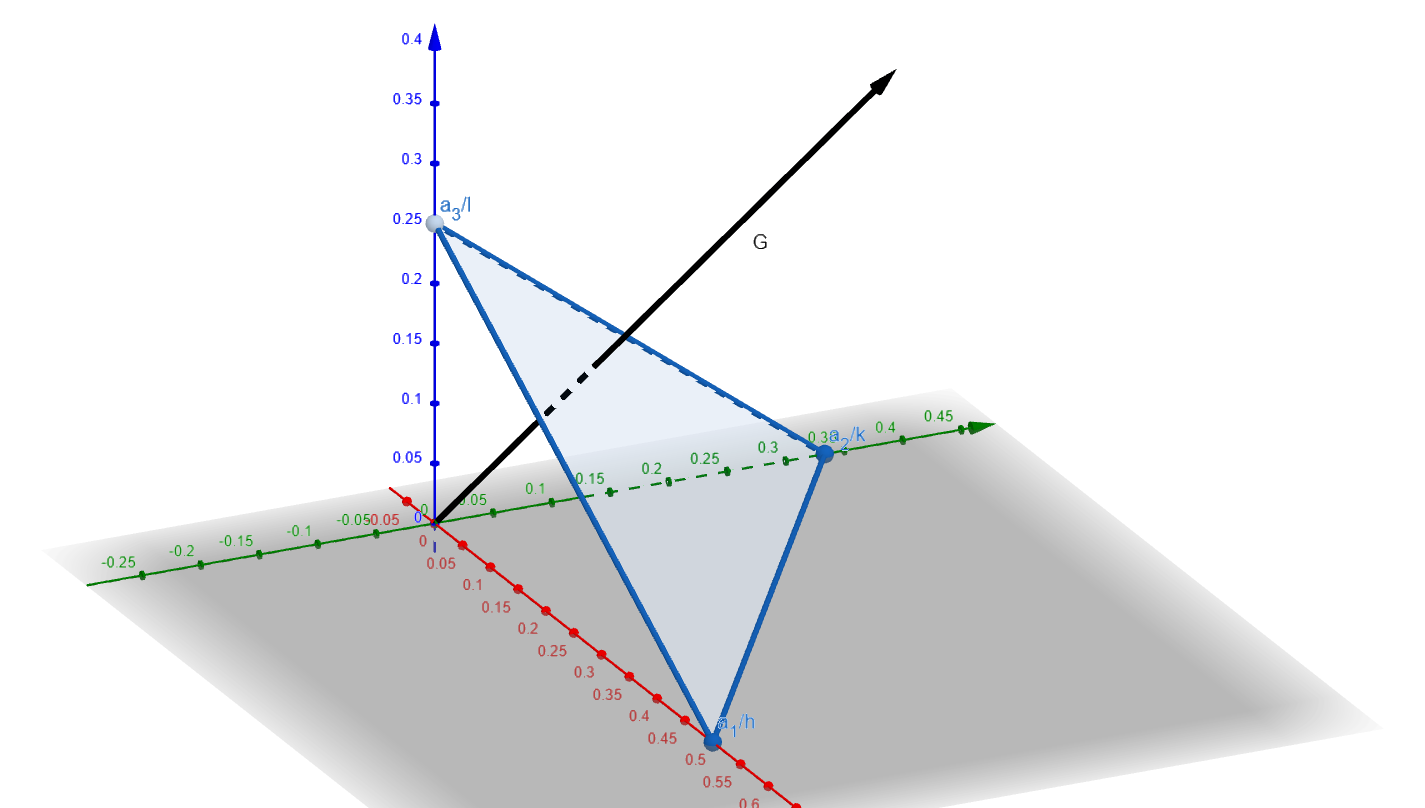
\includegraphics[width=0.7\textwidth]{2_XRD/Graphics/Exercises/MillerPlane.png}
    \caption{Illustration of the $(2,3,4)$ plane}
    \label{fig:MillerPlane}
\end{figure}
\FloatBarrier

Let $\Vec{G} = h\Vec{g}_1 + k\Vec{g}_2 + l\Vec{g}_3$ be a vector of the reciprocal lattice. We can show that $\Vec{G} \perp (h,k,l)$, by looking at the dot product with the basis vectors of the plane:
\begin{align} 
&\begin{cases}
    \Vec{G} \cdot \frac{1}{h} \Vec{a}_1 - \frac{1}{l} \Vec{a}_3 = h \frac{1}{h} \Vec{g}_1 \cdot \Vec{a}_1 - l\frac{1}{l} \Vec{g}_3 \cdot \Vec{a}_3 = 2\pi - 2\pi = 0\\
    \Vec{G} \cdot \frac{1}{k} \Vec{a}_2 - \frac{1}{l} \Vec{a}_3 = k \frac{1}{k} \Vec{g}_2 \cdot \Vec{a}_2 - l\frac{1}{l} \Vec{g}_3 \cdot \Vec{a}_3 = 2\pi - 2\pi = 0
\end{cases}
\end{align}


So $\Vec{G} \perp (h,k,l)$. \\

\textbf{b)} The distance between two neighbouring, parallel planes is the same as the distance from the origin to the first plane $(h,k,l)$. The smallest distance is then given by the length of the vector $\Vec{d}_{hkl} = d_{hkl}\Vec{n}$, where $\Vec{n}$ is the normalized normal vector of the $(h,k,l)$ plane. Using the previous question, we can choose $\Vec{n} = \frac{\Vec{G}}{|\Vec{G}|}$. $d_{hkl}$ is then given by the projection of any of the basis vectors of the direct lattice along the $\Vec{n}$. One can see this when considering the plane $\{\Vec{G}, \frac{1}{h}\Vec{a}_1\}$; the concept is illustrated in figure \ref{fig:Projection}, where $b$ corresponds to $\Vec{G}$ and $a$ corresponds to $\Vec{a}_1$. Using the basis vector $\frac{1}{h} \Vec{a}_1$, we get:
\begin{align}
    d_{hkl} &= \frac{a}{h} \Vec{a}_1 \cdot \frac{\Vec{G}}{|\Vec{G}|} \\
    d_{hkl} &= \frac{1}{|\Vec{G}|}\frac{1}{h}\cdot 2\pi h \\
    d_{hkl} &= \frac{2\pi}{|\Vec{G}|}
\end{align}
\begin{figure}[!ht]
    \centering
    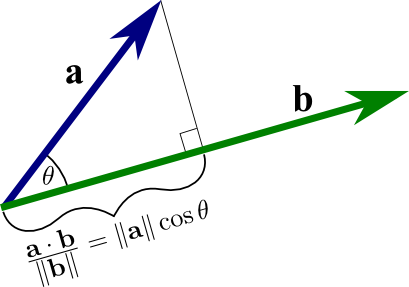
\includegraphics[width=0.5\textwidth]{2_XRD/Graphics/Exercises/Projection.png}
    \caption{Vector projection}
    \label{fig:Projection}
\end{figure}
\FloatBarrier

\textbf{c)} In the case of a cubic lattice, both the direct and reciprocal lattice form an orthogonal base, where $\Vec{a}_i \cdot \Vec{a}_j = a^2 \delta_{ij}$ and $\Vec{g}_i \cdot \Vec{g}_j = \left( \frac{2\pi}{a}\right)^2 \delta_{ij}$. Therefore: $|\Vec{G}| = \sqrt{h^2 \Vec{g}_1 \cdot \Vec{g}_1 + k^2 \Vec{g}_2 \cdot \Vec{g}_2 + l^2 \Vec{g}_3 \cdot \Vec{g}_3} = \frac{2\pi}{a} \sqrt{h^2+k^2+l^2}$. Finally:
\begin{equation}
    d_{hkl} = \frac{a}{\sqrt{h^2+k^2+l^2}}
\end{equation}


\subsection{Problem 2}
The structure factor is given by:
\begin{align}
    S &= \sum_j e^{-i\Vec{G} \cdot \Vec{r}_j} \int_V dV n_j(\rho)e^{-i\Vec{G} \cdot \Vec{\rho}} \\
    \Leftrightarrow S &= \sum_j e^{-i\Vec{G} \cdot \Vec{r}_j} f \\
    \Leftrightarrow S &= \sum_j e^{-i2\pi(hx_j + ky_j + lz_j)}
\end{align}
Where we sum over the j basis vectors with components $(x_j,y_j,z_j)$.
The basis of the fcc structure, in which PdAu crystallizes, are the following: (0,0,0), (0,$\frac{1}{2}$,$\frac{1}{2}$), ($\frac{1}{2}$,0,$\frac{1}{2}$), ($\frac{1}{2}$,$\frac{1}{2}$,0). The structure factor then is:
\begin{equation}
    S = \left[ 1 + e^{-i\pi(k+l)} + e^{-i\pi(h+l)} +e^{-i\pi(h+k)} \right] f
\end{equation}
Now, $e^{-i\pi n} = 1$ for $n$ even, and $e^{-i\pi n} = -1$ for $n$ odd. Since $h,k,l$ are integers, we can distinguish 4 cases:
\begin{enumerate}
    \item $h,k,l$ are all even
    \item $h,k,l$ are all odd
    \item One of $h,k,l$ is odd, and two are even
    \item One of $h,k,l$ is even, and two are odd
\end{enumerate}

Note that the sum of two even numbers is even, the sum of an odd and an even number is odd, and the sum of two odd numbers is even.

The four cases yield a structure factor of:
\begin{enumerate}
    \item $S = (1+1+1+1) f = 4f$
    \item $S = (1+1+1+1) f = 4f$
    \item $S = (1+1-1-1) f = 0$, where $h$ is odd and $k,l$ are even 
    \item $S = (1+1-1-1) f = 0$, where $h$ is even and $k,l$ are odd
\end{enumerate} 
Of course, cases 3 and 4 work for any permutation of evenness of the $h,k,l$. To get reflexes, $S$ must be non-zero, and therefore $h,k,l$ must be either all odd or all even. The first eight sets of $(h,k,l)$ and the associated angles can be found in the table \ref{tab:allowedBraggReflexes}, where Bragg's law was used to get the angle: $\theta = \arcsin{\left(\frac{\lambda}{2a}\sqrt{h^2+k^2+l^2}\right)}$
\begin{table}[!ht]
    \centering
    \begin{tabular}{c|c}
        $(h,k,l)$ & $2\theta$ \\ \hline
        (1,1,1) & 40,1° \\
        (2,0,0) & 46,6° \\
        (2,2,0) & 68,1° \\
        (3,1,1) & 82,1° \\
        (2,2,2) & 86,6° \\
        (4,0,0) & 104,7° \\
        (3,3,1) & 119,3° \\
        (4,2,0) & 124,6° \\
    \end{tabular}
    \caption{The first eight allowed Bragg reflexes}
    \label{tab:allowedBraggReflexes}
\end{table}
\subsection{Problem 3}

\textbf{a)} The amplitude is given by:
\begin{equation}
    F = \sum_m e^{-im(\Vec{a} \cdot \Delta \Vec{k})}
\end{equation}
By identifying $x = e^{-i(\Vec{a} \cdot \Delta \Vec{k})}$ and using the formula: 
\begin{equation}
    \sum_{m=0}^{M-1}x^m = \frac{1-x^M}{1-x}
\end{equation}
We obtain for a system consisting of M lattice points:
\begin{align}
    F &= \sum_{m=0}^{M-1} e^{-im(\Vec{a} \cdot \Delta \Vec{k})} \\ 
    \Leftrightarrow F &= \frac{1-e^{-iM(\Vec{a} \cdot \Delta \Vec{k})}}{1-e^{-i(\Vec{a} \cdot \Delta \Vec{k})}}
\end{align}

\textbf{b)} The complex conjugate of $F$ is:
\begin{equation}
    F^* = \frac{1-e^{iM(\Vec{a} \cdot \Delta \Vec{k})}}{1-e^{i(\Vec{a} \cdot \Delta \Vec{k})}}
\end{equation}
Therefore:
\begin{align}
    |F|^2 &= \frac{1 - e^{iM(\Vec{a} \cdot \Delta \Vec{k})}}{1-e^{i(\Vec{a} \cdot \Delta \Vec{k})}} \cdot \frac{1-e^{-iM(\Vec{a} \cdot \Delta \Vec{k})}}{1-e^{-i(\Vec{a} \cdot \Delta \Vec{k})}} \\
    \Leftrightarrow |F|^2 &= \frac{1 - e^{iM(\Vec{a} \cdot \Delta \Vec{k})} - e^{-iM(\Vec{a} \cdot \Delta \Vec{k})} + e^0}{1 - e^{i(\Vec{a} \cdot \Delta \Vec{k})} - e^{-i(\Vec{a} \cdot \Delta \Vec{k})} + e^0} \\
    \Leftrightarrow |F|^2 &= \frac{2 - (e^{iM(\Vec{a} \cdot \Delta \Vec{k})} + e^{-iM(\Vec{a} \cdot \Delta \Vec{k})})}{2 - ( e^{i(\Vec{a} \cdot \Delta \Vec{k})} + e^{-i(\Vec{a} \cdot \Delta \Vec{k})})}
\end{align}
But $e^{ix}+e^{-ix} = 2\cos(x)$, so this becomes:
\begin{align}
    |F|^2 &= \frac{2-2\cos(M \Vec{a} \cdot \Delta \Vec{k})}{2-2\cos[\Vec{a} \cdot \Delta \Vec{k})} \\
    \Leftrightarrow |F|^2 &= \frac{\sin^2( \frac{1}{2} M \Vec{a} \cdot \Delta \Vec{k})}{\sin^2(\frac{1}{2} \Vec{a} \cdot \Delta \Vec{k})}
\end{align}
Where in the last step we used the trigonometric identity $1 - \cos(2 \theta) = 2\sin^2(\theta)$. \\

\textbf{c)} For $\Vec{a} \cdot \Delta \Vec{k} = 2 \pi h$, $\sin(\frac{1}{2} \Vec{a} \cdot \Delta \Vec{k}) = \sin(\pi h)$. Since h is an integer, $\sin(\pi h) = 0$, but then $|F|^2$ is not defined. We can apply de l'Hôpitals rule twice to find the limit:
\begin{align}
    \lim_{x\rightarrow \pi h} \frac{\sin^2(Mx)}{\sin^2(x)} &= lim_{x\rightarrow \pi h} \frac{[\sin^2(Mx)]''}{[\sin^2(x)]''} \\
    \Leftrightarrow \lim_{x\rightarrow \pi h} \frac{\sin^2(Mx)}{\sin^2(x)} &= lim_{x\rightarrow \pi h} \frac{[2M \cos(Mx)\sin(Mx)]'}{[2\cos(x)sin(x)]'} \\
    \Leftrightarrow \lim_{x\rightarrow \pi h} \frac{\sin^2(Mx)}{\sin^2(x)} &= lim_{x\rightarrow \pi h} \frac{M^2[\cos^2(Mx) - \sin^2(Mx)]}{\cos^2(x) - \sin^2(x)}
\end{align}

Since $M \in \mathbb{N}$ is the amount of lattice points and $h \in \mathbb{N}$, we have: $\cos(hM\pi) = \cos(h\pi) = \pm 1$, and $\sin(hM\pi) = \sin(h\pi) = 0$. Therefore:
\begin{equation}
    \lim_{x\rightarrow \pi h} \frac{\sin^2(Mx)}{\sin^2(x)} = M^2
\end{equation}

\textbf{d)} Let $\Vec{a} \cdot \Delta\Vec{k} = 2\pi h + \epsilon$ such that $\sin\left( \frac{1}{2}M(\Vec{a} \cdot \Delta\Vec{k})\right) = 0$. Using trigonometric addition formulas, it follows that:
\begin{align}
    &\sin \left( \frac{M}{2} 2\pi h + \frac{M\epsilon}{2} \right) = 0 \\
    \Leftrightarrow  &\sin(hM\pi) \cos \left( \frac{M\epsilon}{2} \right) + \cos(hM\pi) \sin \left( \frac{M\epsilon}{2} \right) = 0 \\
    \Leftrightarrow &\cos(hM\pi) \sin \left( \frac{M\epsilon}{2} \right) = 0
\end{align}
Since $\cos(hM\pi) = \pm 1$ this is only true if:
\begin{align}
    &\sin \left( \frac{M\epsilon}{2} \right) = 0 \\
    \Rightarrow \ &\frac{M\epsilon}{2} = n\pi, \quad n\in \mathbb{Z} \\
    \Leftrightarrow \ &\epsilon = \frac{2 \pi n}{M}
\end{align}
Thus yielding for the first zero of $|F|^2$ at $n = 1$:
\begin{equation}
    \epsilon = \frac{2\pi}{M}
\end{equation}

\textbf{e)} Using $\Vec{a} \cdot \Delta \Vec{k} = \frac{4 \pi a}{\lambda}\sin(\theta)$ we get the following plots for $M = 10,100,1000$:
\begin{figure}[!ht]
    \begin{subfigure}{0.5\textwidth}
        \centering
        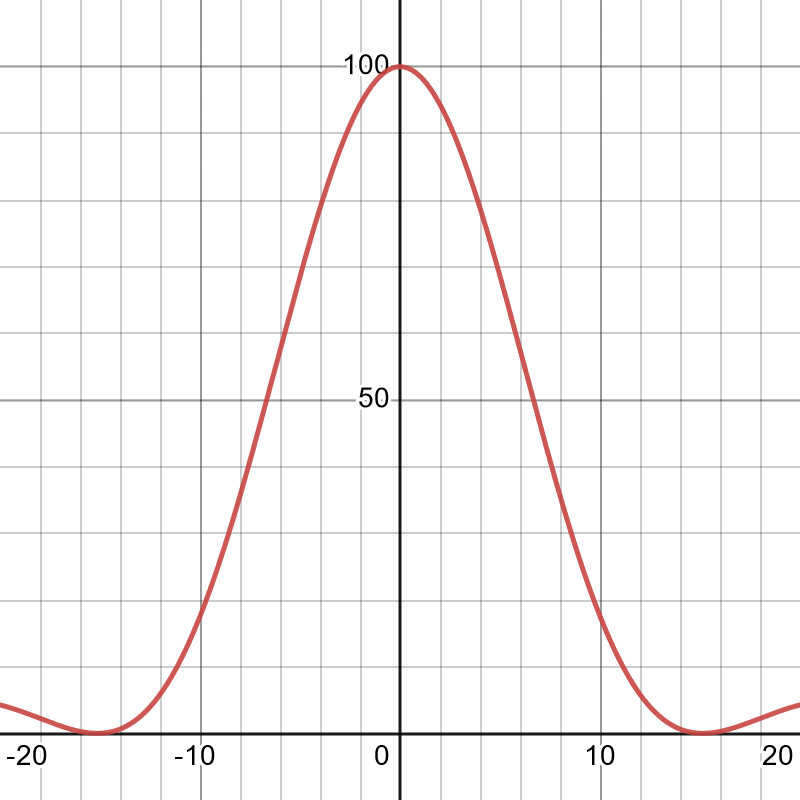
\includegraphics[width=\textwidth]{2_XRD/Graphics/Exercises/M=10.png}
        \caption{$M=10$}
        \label{fig:subM10}
    \end{subfigure}
    \begin{subfigure}{0.5\textwidth}
        \centering
        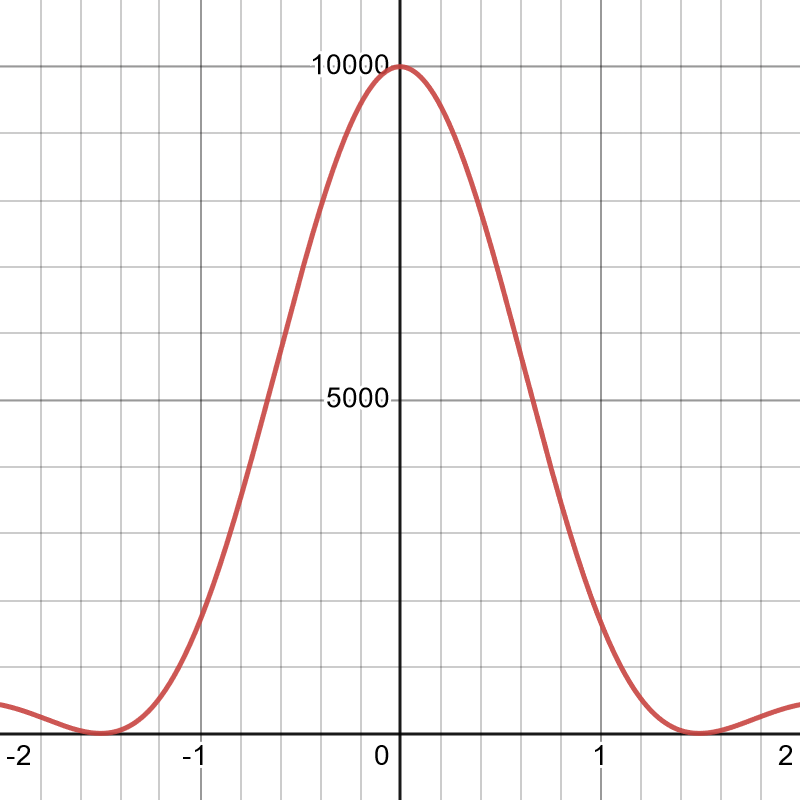
\includegraphics[width=\textwidth]{2_XRD/Graphics/Exercises/M=100.png}
        \caption{$M=100$}
        \label{fig:subM100}
    \end{subfigure}

    \begin{subfigure}[c]{0.5\textwidth}
        \centering
        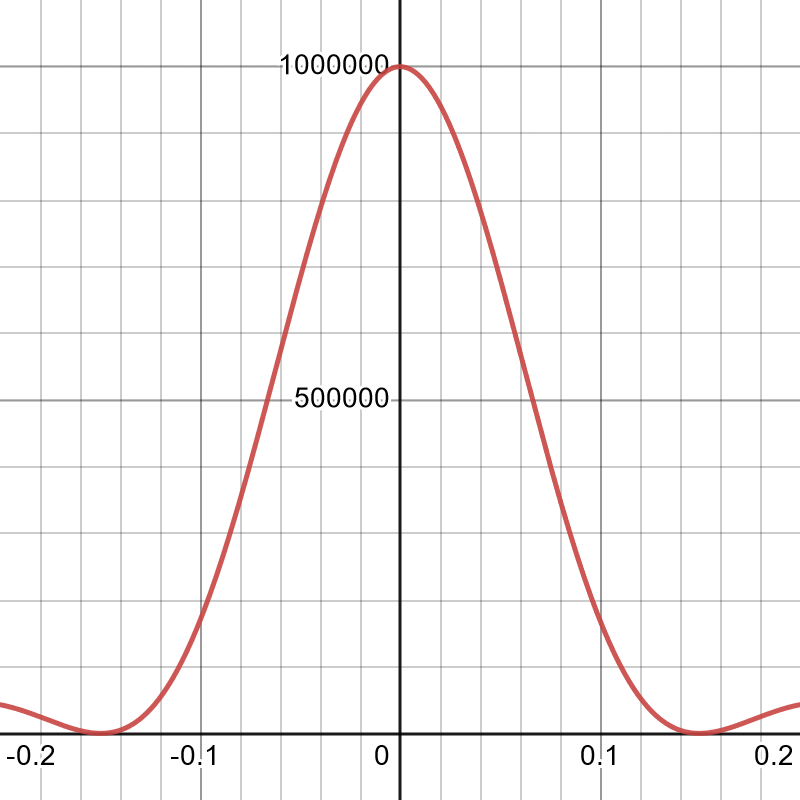
\includegraphics[width=\textwidth]{2_XRD/Graphics/Exercises/M=1000.png}
        \caption{$M=1000$}
        \label{fig:subM1000}
    \end{subfigure}
    \label{fig:plotF*F}
    \caption{Plots of $|F|^2$ against $\theta$ for various values of $M$}
\end{figure}
\FloatBarrier

\subsection{Problem 4}
Bragg's law is stated as: 
\begin{equation}
    2d\sin(\theta) = n\lambda
\end{equation}

\textbf{a)} Using problem 1, Bragg's law becomes:
\begin{equation}
    \frac{2a}{\sqrt{h^2+k^2+l^2}} \sin(\theta) = n\lambda
\end{equation}
Solving for $a$, we obtain:
\begin{align}
    a &= \frac{n\lambda \sqrt{h^2+k^2+l^2}}{2\sin(\theta)} \\ 
    \Leftrightarrow a &= \Lambda\frac{1}{\sin(\theta)}
\end{align}
where $\Lambda = \frac{1}{2} n\lambda \sqrt{h^2+k^2+l^2}$.

We are interested in $\frac{\partial a}{\partial2\theta}$, and we do the substitution $v = 2\theta \Leftrightarrow \theta = \frac{v}{2}$. Thus:
\begin{align}
    \frac{\partial a}{\partial2\theta} &= \frac{\partial }{\partial v} \left[ \Lambda\frac{1}{\sin(\frac{v}{2})} \right] \\
    \Leftrightarrow \frac{\partial a}{\partial2\theta} &= \Lambda \frac{1}{2} \frac{\cos(\frac{v}{2})}{\sin^2(\frac{v}{2})} \\
    \Leftrightarrow \frac{\partial a}{\partial2\theta} &= \Lambda \frac{1}{2} \frac{\cos(\theta)}{\sin^2(\theta)}
\end{align}
Dividing by $a$ yields:
\begin{align}
    \frac{1}{a}\frac{\partial a}{\partial2\theta} &= \frac{1}{2 \tan(\theta)} \\
    \Rightarrow \delta2\theta &= 2\tan(\theta)\frac{\delta a}{a}
\end{align}
Since $0<\theta< \pi$, $\tan(\theta) > 0$, so we finally get the relation:
\begin{equation}
    \left|\delta2\theta\right| = 2\tan(\theta)\left|\frac{\delta a}{a}\right|
\end{equation}

\textbf{b)} Using the parametrization $s = \frac{2}{\lambda} \sin(\theta)$, we get the expression $\sin(\theta) = \frac{s \lambda}{2}$, and Bragg's law reduces to:
\begin{align}
    sd &= n \\
    \Leftrightarrow a &= \frac{n}{s} \sqrt{h^2+k^2+l^2} \\
    \Leftrightarrow a &= \frac{\alpha}{s}
\end{align}
With $\alpha = n\sqrt{h^2+k^2+l^2}$. Using the same method as in the previous part, we obtain:
\begin{align}
    \frac{1}{a} \frac{\partial a}{\partial s} &= \frac{s}{\alpha} \frac{-\alpha}{s^2} \\ 
    \Leftrightarrow \frac{1}{a} \frac{\partial a}{\partial s} &= \frac{-1}{s} 
\end{align}
And finally, since $0<\theta<\pi$, we have $0<s<\frac{2}{\lambda}$. Therefore:
\begin{equation}
    \left| \delta s\right| = s \left| \frac{\delta a}{a} \right|    
\end{equation}

\newpage

\section{Appendix: Error calculation}

The general formula for calculating the uncertainty $\Delta q$ of a quantity $q = f(x_1, \dots, x_n)$, with uncertainties $\Delta x_i$ in the arguments, is given by \cite{ErrorPropagation}:
\begin{equation}
    \Delta q = \sqrt{ \sum_{i=1}^n \left( \frac{\partial f}{\partial x_i} \Delta x_i \right)^2}
\end{equation}

The error calculations are detailed in this section.

\subsection{Lattice constant}

The error $\Delta a$ on $a$ is then given by:
\begin{equation}
    \Delta a = \frac{\lambda \sqrt{h^2+k^2+l^2}}{2} \left| \frac{\cos(\theta)}{\sin^2(\theta)}\right| \Delta \theta
\end{equation}

In order to identify the error on $\frac{\cos^2(\theta)}{\sin(\theta)}$, we do the following quick calculation:
\begin{align}
    \frac{\partial}{\partial 2\theta} \frac{\cos^2(\theta)}{\sin(\theta)} &= \frac{\partial}{\partial v} \frac{\cos^2(\frac{v}{2})}{\sin(\frac{v}{2})} \\
    \Leftrightarrow \frac{\partial}{\partial 2\theta} \frac{\cos^2(\theta)}{\sin(\theta)} &= \frac{-\sin(\frac{v}{2})\cos(\frac{v}{2}) \cdot \sin(\frac{v}{2}) - \frac{1}{2} \cos^2(\frac{v}{2}) \cdot \cos(\frac{v}{2})}{\sin^2(\frac{v}{2})} \\
    \Leftrightarrow \frac{\partial}{\partial 2\theta} \frac{\cos^2(\theta)}{\sin(\theta)} &= -\cos(\frac{v}{2}) - \frac{\cos^3(\frac{v}{2})}{2 \sin^2( \frac{v}{2})} \\
    \Leftrightarrow \frac{\partial}{\partial 2\theta} \frac{\cos^2(\theta)}{\sin(\theta)} &= -\cos(\frac{v}{2}) - \frac{\cos(\frac{v}{2})(1-\sin^2(\frac{v}{2}))}{2 \sin^2( \frac{v}{2})} \\
    \Leftrightarrow \frac{\partial}{\partial 2\theta} \frac{\cos^2(\theta)}{\sin(\theta)} &= -\cos(\frac{v}{2}) - \frac{\cos(\frac{v}{2})}{2\sin^2(\frac{v}{2})} + \frac{1}{2} \cos(\frac{v}{2}) \\
    \Leftrightarrow \frac{\partial}{\partial 2\theta} \frac{\cos^2(\theta)}{\sin(\theta)} &= - \frac{1}{2} \cos(\frac{v}{2}) - \frac{\cos(\frac{v}{2})}{2\sin^2(\frac{v}{2})} \\
    \Leftrightarrow \frac{\partial}{\partial 2\theta} \frac{\cos^2(\theta)}{\sin(\theta)} &= - \frac{1}{2} \cos(\theta) - \frac{\cos(\theta)}{2\sin^2(\theta)} \\
\end{align}

Finally, we obtain: 
\begin{equation}
    \Delta \left( \frac{\cos^2(\theta)}{\sin(\theta)} \right) = \frac{1}{2} \left| \left( \cos(\theta) + \frac{\cos(\theta)}{\sin^2(\theta)} \right)  \right| \Delta 2 \theta
\end{equation}


\subsection{Caglioti function}

The error $\Delta \tan(\theta)$ is determined by:

\begin{equation}
    \Delta \tan(\theta) = (1+\tan^2(\theta)) \Delta \theta
\end{equation}

\subsection{Instrumental broadening}

Since the instrumental broadening is given by:
\begin{equation}
    (\delta 2 \theta)_{inst} = \sqrt{A+B\tan(\theta)+C\tan^2(\theta)}
\end{equation}

We can determine the uncertaity:
\begin{equation}    
    \Delta (\delta 2 \theta)_{inst} = \sqrt{\left( \frac{\partial (\delta 2 \theta)_{inst}}{\partial A} \Delta A \right)^2 + \left( \frac{\partial (\delta 2 \theta)_{inst}}{\partial B} \Delta B \right)^2 + \left( \frac{\partial (\delta 2 \theta)_{inst}}{\partial C} \Delta C \right)^2 + \left( \frac{\partial (\delta 2 \theta)_{inst}}{\partial \theta} \Delta \theta \right)^2}
\end{equation}

It is easy to verify that:
\begin{equation}
    \begin{cases}
        \frac{\partial (\delta 2 \theta)_{inst}}{\partial A} = \frac{1}{2(\delta 2 \theta)_{inst}} \\
        \frac{\partial (\delta 2 \theta)_{inst}}{\partial B} = \frac{\tan(\theta)}{2(\delta 2 \theta)_{inst}} \\
        \frac{\partial (\delta 2 \theta)_{inst}}{\partial C} = \frac{\tan^2(\theta)}{2(\delta 2 \theta)_{inst}} \\
        \frac{\partial (\delta 2 \theta)_{inst}}{\partial \theta} = \frac{(1+\tan^2(\theta))(B + C\tan(\theta))}{2(\delta 2 \theta)_{inst}}
    \end{cases}
\end{equation}

Putting everything back together, we obtain:
\begin{equation}
    \Delta (\delta 2 \theta)_{inst} = \frac{1}{2(\delta 2 \theta)_{inst}}\sqrt{ \left(\Delta A \right)^2 + \left( \tan(\theta) \Delta B \right)^2 + \left( \tan^2(\theta) \Delta C \right)^2 + \left( (1+\tan^2(\theta))(B + C\tan(\theta)) \Delta \theta \right)^2}
\end{equation}

Finally, we neglect the angular uncertainty and thus the uncertainty is:
\begin{equation}
    \Delta (\delta 2 \theta)_{inst} = \frac{1}{2(\delta 2 \theta)_{inst}}\sqrt{ \left(\Delta A \right)^2 + \left( \tan(\theta) \Delta B \right)^2 + \left( \tan^2(\theta) \Delta C \right)^2}
\end{equation}

\subsection{Corrected broadening}

The corrected broadening is given by:
\begin{equation}
    (\delta 2 \theta)_{corr} = (\delta 2 \theta) - (\delta 2 \theta)_{inst} 
\end{equation}

The resulting error is then simply:
\begin{equation}
    \Delta (\delta 2 \theta)_{corr} = \sqrt{[\Delta (\delta 2 \theta)]^2 + [\Delta (\delta 2 \theta)_{inst}]^2}
\end{equation}
    
\subsection{Change of variable}

When applying the change of variable:
\begin{equation}
    s = \frac{2\sin(\theta)}{\lambda}
\end{equation}

The error propagation yields:
\begin{equation}
    \Delta s = \frac{2}{\lambda} |\cos(\theta) \Delta \theta|
\end{equation}

Since $\Delta \theta = \frac{1}{2} \Delta (2\theta)$, this becomes:
The error propagation yields:
\begin{equation}
    \Delta s = \frac{1}{\lambda} |\cos(\theta) \Delta (2\theta)|
\end{equation}

The peak broadening is then given by:
\begin{equation}
    \delta s = \frac{\cos(\theta)}{\lambda} (\delta 2\theta)_{corr}
\end{equation}

Resulting in an uncertainty of:
\begin{equation}
    \Delta \delta s = \frac{1}{\lambda}\sqrt{[\sin(\theta) (\delta 2\theta)_{corr} \Delta \theta]^2 + [\cos(\theta) \Delta (\delta 2 \theta)_{corr}]^2}
\end{equation}

Then, we obtain:
\begin{equation}
    \Delta (s^2) = 2 s \Delta s
\end{equation}

and similarly:
\begin{equation}
    \Delta [(\delta s)^2] = 2 \delta s \Delta (\delta s)
\end{equation}

For Lorentzians, the error is given by:
\begin{equation}
    \Delta (\delta 2 \theta)_{corr} = \sqrt{(\Delta (\delta 2\theta)_{tot})^2 + (\Delta (\delta 2\theta)_{inst})^2}
\end{equation}

Whereas for Gaussians, the error is given by:
\begin{equation}
    \Delta (\delta 2 \theta)_{corr} = \sqrt{[2\Delta (\delta 2 \theta)_{tot}]^2 + [2\Delta (\delta 2 \theta)_{inst}]^2}
\end{equation}

\subsection{Strain and crystallite size}

\subsubsection{Lorentzian}

We have:
\begin{equation}
    \begin{cases}
        m = 2e \Leftrightarrow e = \frac{m}{2} \\
        p = \frac{6}{5D} \Leftrightarrow D = \frac{6}{5p}
    \end{cases}
\end{equation}

Therefore: 
\begin{equation}
    \begin{cases}
        \Delta e = \frac{\Delta m}{2} \\
        \Delta D = \frac{6 \Delta p}{5 p^2}
    \end{cases}
\end{equation}

\subsubsection{Gaussian}

We have:
\begin{equation}
    \begin{cases}
        m = (2e)^2 \Leftrightarrow e = \frac{\sqrt{m}}{2} \\
        p = (\frac{6}{5D})^2 \Leftrightarrow D = \frac{6}{5\sqrt{p}}
    \end{cases}
\end{equation}

Therefore: 
\begin{equation}
    \begin{cases}
        \Delta e = \frac{\Delta m}{4 \sqrt{m}} \\
        \Delta D = \frac{3 \Delta p}{5 p^{\frac{3}{2}}}
    \end{cases}
\end{equation}

\printbibliography

\end{document}